\documentclass[smallextended]{svjour3}

\usepackage{amssymb}
\usepackage{times}
\usepackage{ifthen}
%\usepackage[pdftex]{graphicx}
\usepackage{url}
\usepackage{soul}
\usepackage[dvipsnames,usenames]{color}
\usepackage{colortbl}
\usepackage{tabularx}
\usepackage{hanging}
\usepackage{xspace}
\usepackage{wasysym}
\usepackage{multirow}
\usepackage{topcapt}
\usepackage{threeparttable}
\usepackage{pdfpages}
\usepackage[bookmarksopen=true, 
			colorlinks=true, 
			linkcolor=blue, 
			citecolor=OliveGreen, 
			urlcolor=blue]{hyperref}			% should come last

\usepackage{breakurl}
\usepackage{caption}
\DeclareCaptionType{copyrightbox}			
%\usepackage[font=small,labelsep=none]{caption}
%\pdfpagewidth=8.5in
%\pdfpageheight=11in

\graphicspath{{figs/}}
\DeclareGraphicsExtensions{.pdf, .png, .ps, .eps}   % NOT .jpg  because it throws away the detail.

\definecolor{OliveGreen}    {cmyk}{0.64,0,0.95,0.40}


\makeatletter
\def\url@leostyle{%
  \@ifundefined{selectfont}{\def\UrlFont{\sf}}{\def\UrlFont{\small\sffamily}}}
\makeatother
\urlstyle{leo} 

\newcommand\gc{\rowcolor[rgb]{0.93,0.93,0.93}}

\newcommand{\squishlist}{
	\vspace{0mm}
   \begin{list}{$\bullet$}
    { \setlength{\itemsep}{0pt}      \setlength{\parsep}{3pt}
      \setlength{\topsep}{3pt}       \setlength{\partopsep}{0pt}
      \setlength{\leftmargin}{1.5em} \setlength{\labelwidth}{1em}
      \setlength{\labelsep}{0.5em} } }

\newcommand{\squishend}{
    \end{list}  }

\newcommand\discovery{peer interaction\xspace}
\newcommand\Discovery{Peer interaction\xspace}
\newcommand\DisCovery{Peer Interaction\xspace}
\newcommand\DISCOVERY{PEER INTERACTION\xspace}

\newcommand\discpush{peer recommendation\xspace}
\newcommand\DiscPush{Peer Recommendation\xspace}

\newcommand\discpull{peer observation\xspace}
\newcommand\Discpull{Peer observation\xspace}
\newcommand\DiscPull{Peer Observation\xspace}

\newcommand\context{mode\xspace}
\newcommand\contexts{modes\xspace}
\newcommand\Contexts{Modes\xspace}


\newcommand{\subject}[1]{\textsc{#1}}
\newcommand{\asub}{{\subject{Zac}}\xspace}
\newcommand{\bsub}{{\subject{Rob}}\xspace}
\newcommand{\csub}{{\subject{Eli}}\xspace}
\newcommand{\dsub}{{\subject{Ben}}\xspace}
\newcommand{\esub}{{\subject{Val}}\xspace}
\newcommand{\fsub}{{\subject{Art}}\xspace}
\newcommand{\gsub}{{\subject{Hao}}\xspace}
\newcommand{\hsub}{{\subject{Fez}}\xspace}
\newcommand{\isub}{{\subject{Gus}}\xspace}
\newcommand{\jsub}{{\subject{Yit}}\xspace}
\newcommand{\ksub}{{\subject{Cal}}\xspace}
\newcommand{\lsub}{{\subject{Kai}}\xspace}
\newcommand{\msub}{{\subject{Don}}\xspace}
\newcommand{\nsub}{{\subject{Del}}\xspace}
\newcommand{\osub}{{\subject{Ken}}\xspace}
\newcommand{\psub}{{\subject{Hal}}\xspace}
\newcommand{\qsub}{{\subject{Enu}}\xspace}
\newcommand{\rsub}{{\subject{Gil}}\xspace}

\newcommand{\shortName}[1]{{\fontsize{6}{6}\textsf{\framebox[6mm]{#1}}}}
\newcommand{\asss}{{\shortName{\asub}}}
\newcommand{\bsss}{{\shortName{\bsub}}}
\newcommand{\csss}{{\shortName{\csub}}}
\newcommand{\dsss}{{\shortName{\dsub}}}
\newcommand{\esss}{{\shortName{\esub}}}
\newcommand{\fsss}{{\shortName{\fsub}}}
\newcommand{\gsss}{{\shortName{\gsub}}}
\newcommand{\hsss}{{\shortName{\hsub}}}
\newcommand{\isss}{{\shortName{\isub}}}
\newcommand{\jsss}{{\shortName{\jsub}}}
\newcommand{\ksss}{{\shortName{\ksub}}}
\newcommand{\lsss}{{\shortName{\lsub}}}
\newcommand{\msss}{{\shortName{\msub}}}
\newcommand{\nsss}{{\shortName{\nsub}}}
\newcommand{\osss}{{\shortName{\osub}}}
\newcommand{\psss}{{\shortName{\psub}}}
\newcommand{\qsss}{{\shortName{\qsub}}}
\newcommand{\rsss}{{\shortName{\rsub}}}

\newboolean{hidecomments}
\setboolean{hidecomments}{true}
\ifthenelse{\boolean{hidecomments}}
{\newcommand{\nb}[2]{}}
{\newcommand{\nb}[2]{
    \fbox{\bfseries\sffamily\scriptsize#1}
    {\sf\small$\blacktriangleright$
      {#2} $\blacktriangleleft$}}}
\newcommand\gcm[1]{\nb{GCM}{#1}}
\newcommand\emh[1]{\nb{EMH}{#1}}
\newcommand\idrg[1]{\nb{IDRG}{#1}}
\newcommand\jh[1]{\nb{JH}{#1}}
  
\hyphenation{Petch-arat}

\begin{document}

\clubpenalty=10000
\widowpenalty = 10000


\title{How Do Users Discover New Tools\\in Software Development and Beyond?}

\author{Emerson Murphy-Hill         \and
        Da Young Lee \and
        Gail~C.~Murphy \and
        Joanna McGrenere
}

\authorrunning{Murphy-Hill, Lee, Murphy, and McGrenere} % if too long for running head

\institute{Emerson Murphy-Hill and Da Young Lee\at
              Department of Computer Science\\North Carolina State University\\Raleigh, USA \\
              \email{\{emerson,dlee\}@csc.ncsu.edu}           %  \\
           \and
           	  Gail C. Murphy and Joanna McGrenere\at 
           	  Department of Computer Science\\University of British Columbia\\Vancouver, Canada \\
              \email{\{murphy,joanna\}@cs.ubc.ca}           %  \\
}

\maketitle

\begin{abstract}

Computer users rely on software tools such as browser tab controls and spell checkers to work effectively 
and efficiently, but it is difficult for users to be aware of all the tools that might be useful to them. 
While there are several potential technical solutions to this difficulty, we know little about social solutions, such as one user telling a peer about a tool.
To explore these social solutions, we conducted two studies, an interview study and a diary study.
The interview study describes a series of interviews with 18 programmers in industry to explore how tool discovery takes place. 
To broaden our findings to a wider group of software users, 
we then conducted a diary study of 76 software users in their workplaces.
One finding was that social learning of software tools, while sometimes effective, is rare;
software users appear to discover 
tools from peers only once every few months.
We describe several implications of our findings, such as that discovery from peers can 
be enhanced by improving software users' ability to communicate openly and concisely about tools.

\keywords{discovery \and learning \and programmers \and programming tools}

\end{abstract}


%------------------------------------------------------------------------- 
\section{Introduction}\label{sec:intro}

\noindent
Software tools such as the functionality to correct grammar in Microsoft
Word~\cite{word} or to recover recently closed tabs in Mozilla Firefox~\cite{firefox}, allow users to 
perform their tasks more efficiently and do things they were unable to do
previously.
We define a `tool' broadly as any software that helps a user accomplish a task.
This includes standalone programs like development environments 
and desktop publishing software,
but also includes features or commands in those environments, 
like source code formatters and spell checkers.

Users have difficulty discovering tools that might be
useful to them.
When we say that a user discovers a tool, we mean that she becomes
aware of that tool.
For example, when Grossman and colleagues conducted a study of 10 users of
a computer-aided drafting application, they found that a ``typical problem was
that users were not aware of a specific tool or operation which was available for
use''~\cite{grossman09}.
As another example, Campbell and Miller have noted that awareness is a problem
in integrated development environments that are used by
programmers~\cite{campbell08}. 
It is arguable that in any sophisticated software, many
users will remain unaware of the full range of tools available.

The focus of this paper is on \emph{social solutions} to the problem of lack of
awareness, namely where a user learns about a tool from another user. 
There has been relatively little research into such solutions. 
In contrast, there has been
considerable research into technical solutions.
Some applications attempt to solve this problem with tip-of-the-day messages or
role-based customizations of the user interface~\cite{findlater08}.
Researchers have proposed other technical solutions as well,
such as recommender systems that suggest tools that you are not currently 
using~\cite{linton,maltzahn,matejka09}.
These systems attempt to assist or replicate users helping other users, 
such as Maltzahn's ToolBox~\cite{maltzahn}, which helps Unix users find new commands based on the
commands that their coworkers are using.
As Fischer and colleagues point out, these technical solutions ``should guide
and advise an user [sic] similar to a knowledgeable colleague or
assistant''~\cite[p.~115]{fischer84}, so understanding how such knowledge is
transferred socially should help inform the design of such technical solutions.

To illustrate what we mean by social solutions to the awareness problem, let us
give an example drawn from one of the studies that we describe in this paper.
\hsub is a programmer who often works with another programmer named
\psub. While using a remote screen-sharing session together, \hsub noticed that \psub
did something to make some text move around in their shared vim
editor. 
Figure~\ref{fig:pairRemoting} shows an exchange that followed in an
instant-messaging session.
In this session, \hsub gained awareness of a tool that he later found very
useful.
We call this \context of discovery \textbf{\discovery,} where users discover
tools from their peers during normal work activities.

\begin{figure}[t]
	\arrayrulecolor[gray]{0.8} %line color
	\renewcommand{\arraystretch}{1.4} 
	\centering
	\begin{tabularx}{\linewidth}{|llX|}	
		
\gc		(02:02:21 PM)&\hsub:&Hold on.\\
\gc		(02:02:23 PM)&\hsub:&What did you just do?\\
		(02:02:39 PM)&\psub:&Replace the first three 
						     arguments with a combined one. \\	
\gc		(02:02:39 PM)&\hsub:&How'd you do that delete?\\
		(02:02:45 PM)&\psub:&Oh. 'd\%'\\
\gc		(02:02:59 PM)&\hsub:&But then you deleted the -$>$ too.\\
		(02:03:19 PM)&\psub:&Yeah, it scans forward for the next open thingy,
							 then to the matching close thingy.\\
		\hline
        
	\end{tabularx}
	\caption{During a remote screen sharing session, a snippet of an instant-messaging log shows
	where one user learns about a software tool from another user.}\label{fig:pairRemoting}
\end{figure}

In this paper, we investigate the intertwined social and technical contexts that allowed
\hsub to discover a useful tool from a peer, yet sometimes
make it difficult for other software users to discover other useful tools.
%What are the key differences in the social and technical contexts that allow
%\hsub to discover useful tools when programming with a peer, yet often
%disallow \csub to discover them through microblogs?
In our first study, we explore these contexts by focusing on programmers, both because we are conversant
with the tools that programmers use and because the range of tools available to programmers is so wide.
In our second study, we extend our participant group to software users in general
to compare and contrast our results from the first study.
The technical contexts we explore in this paper are complex software environments, such as 
programming editors and desktop web browsers.
The social contexts we explore are broad, representing many different workplace environments where 
software users collaborate to discover new tools.
Our long-term research goal is to encourage all kinds of software users to 
discover useful tools more successfully, more frequently.

This paper is an extension of a conference paper presented at CSCW 2011~\cite{murphy-hill11:peer},
where we presented the first study.
In that paper, we made three primary contributions:

\squishlist
  \item an enumeration of the \contexts in which programmers discover new tools;
  \item a characterization of \discovery, a \context of discovery where
  		programmers learn about the existence of new tools from peers; and
  \item evidence that \discovery may be the most effective way for
  		programmers to learn new tools, yet it appears to occur infrequently.
\squishend
%  \item implications for how the social process of \discovery can be
%  		fostered so that it can occur more frequently in the future; and  		 

\noindent
In this paper, we additionally describe a diary study that provides a broader account
of tool discovery, adding two additional contributions:

\squishlist
  \item a comparison between tool discovery in software development and tool
  		discovery for other software users engaged in other kinds of information work; and
  \item a more accurate quantification over a wider domain of tool use 
  		of how often various \contexts of tool discovery,
  		including \discovery, occur in practice.
\squishend



\section{Related Work}\label{sec:relatedWork}

\noindent
We base our work on several existing theories of adoption and
learning, described in several areas of related work.

\subsection{Tool Discoverability}\label{sec:terminology}

\noindent
Two existing studies have looked at tool discoverability directly.
First, in prior work we interviewed software developers to 
understand why they adopt security tools~\cite{xiao}.
Although that study is similar to the first study we report in this paper, 
the present paper seeks to understand
tool adoption in a wider context: beyond security tools and beyond software developers.
Second, the diary study that we present in this paper is similar to 
a study performed by Rieman~\cite{rieman}.
Rieman asked 14 computer users to keep a diary of
daily activities and specific learning events.
The main difference between Rieman's diary study and our
own is that we seek to characterize how users discover tools
that they were not intending to learn (we call this \emph{serendipitous} discovery), 
whereas Rieman largely reported on how users purposefully sought out help
on how to complete a task with tools (we call this \emph{purposeful} discovery).
Of the 60 tool discovery events recorded by Rieman, 
only 7 were serendipitous; in contrast, in our analysis of our diary
study we describe 45 reports of exclusively serendipitous tool discoveries.

\subsection{Diffusion of Innovations}

\noindent Diffusion of Innovations is a theory that attempts to explain ``the
process by which an innovation is communicated through certain channels over
time among the members of a social system''~\cite{rogers03}.
Typical studies of Diffusion of Innovations include research about internet use,
hybrid corn in the US, and water sanitation in developing countries.
Similar models have been developed for more specific contexts, including 
the Technology Acceptance Model~\cite{DAVI89,VENK00}, Perceived
Characteristics of Innovating~\cite{MOOR91}, Theory of Planned
Behavior~\cite{AJZE91}, and Model of Personal Computers
Utilization~\cite{THOM91}.
Both studies presented in this paper can be considered Diffusion of Innovation
studies that investigate tool discovery.

Several studies have investigated Diffusion of Innovations in
other software engineering contexts.
For example, Fichman and Kemerer describe how relational databases, programming
languages, and Computer-Aided Software/Systems Engineering (CASE) tools are
acquired and deployed in organizations~\cite{fichman99}. 
Similarly, Iivari described a study that suggests that the reason that
companies do not use CASE tools is because of a lack of management support, a 
lack of perceived advantage, and a lack of freedom of choice~\cite{iivari}.
Such research addresses critical issues, but it also
tends to focus on tools that require a significant investment of time 
or money, and thus warrant careful organizational consideration of whether or
not to adopt. 
In contrast, our research seeks to investigate a broad spectrum of tools, all
the way down to simple tools such as source code formatters, which likely require
significantly less consideration from individual programmers than higher-level
tools. 
Thus, while that existing research has helped to determine
how and why development environments have been adopted by organizations, our
research additionally helps explain how and why software users discover tools within
those environments.

\subsection{Social Learning}

\noindent
Tool discovery is closely related to learning, in that discovery can be thought 
of as the part of certain learning theories.

One related theory is Lave and Wenger's situated learning~\cite{lave}, where the learning
occurs in the same place that the learning is used, a more general form of
\discovery.
For instance, apprenticeships are a kind of situated learning. 
Whereas Lave and Wegner have largely studied a fixed teacher-learner
relationship, our research on \discovery is on learning in peer-peer relations. 
Despite a focus on teacher-learner relationships, Lave and Wegner imply that
there is significant potential in peer-peer learning: ``There is anecdotal
evidence\ldots that where circulation of knowledge among peers and near-peers
is possible, it spreads exceedingly rapidly and effectively''~\cite{lave}.
Our studies confirm this implication.

Another type of learning is Marsick and Watkin's informal and incidental
learning, where learning happens as a by-product of other
activities~\cite{marsick01}. 
Marsick and Watkins note that with this type, ``control of learning
rests primarily in the hands of the learner''~\cite{marsick01}.
In contrast, in \discovery, learning is controlled by two people. 
We extend research on informal and incidental learning 
into the domain of software.

The zone of proximal development~\cite{vygotsky}, the distance between
what a learner can do on her own and what she can do with help from
more capable peers, is also related in that learning about tools during
\discovery is within the zone of proximal development.
While the zone of proximal development has applied to help people learn
while using software~\cite{borthick,crook,luckin},
we do not believe it has been applied to understanding how people
learn software itself.

% Constructionist learning~\cite{papert}, where a person learns by
% constructing a mental model of a thing by manipulating that thing,
% is also somewhat related\ldots eh, not seeing the connection.

Yet another related concept is over-the-shoulder learning, where colleagues help
each other informally to use a computer application~\cite{twidale05}; 
over-the-shoulder learning is closely related to \discovery in that
they both occur among peers and both in a technology setting.
The difference is that work on over-the-shoulder learning, as 
defined by Twidale~\cite{twidale05}, is focused on situations where the learner purposefully asks for help,
not in situations when the learner discovers a new tool serendipitously.
%this is a generalization; but I can only find one empr. OTSL paper; cited
In \discovery, the learner does not initially know that she might find a tool
useful.

\subsection{Learning During Programming}

Some existing work has explored software tool learning specifically in the domain
of programming, such as Cockburn and Williams description
of learning of tools from peers during pair programming~\cite{cockburn00}.
Specifically, they describe \discovery happening during pair programming, 
when two programmers work on the same programming task at the same computer.
In such situations, the ``driver'' is at the keyboard, and the ``navigator'' is
sitting beside the driver, observing and making suggestions~\cite{cockburn00}.
We hypothesize that a programmer may discover a new tool in either role:
\begin{itemize}
\item
The driver may discover a new tool when the navigator says 
something like, ``you could really use tool X instead.'' 
We call this \textbf{\discpush.}
\item
The navigator may discover a new tool when observing the driver using the tool,
saying something like, ``how did you do that?'' 
We call this \textbf{\discpull.}
\end{itemize}

\noindent
Note that, in both cases, the learner did not expect beforehand to 
learn something new.
Thus, in this paper, we focus on unexpected learning events, 
where a learner does not realize she needs a tool before she 
learns about it.

In pair programming, Cockburn and Williams suggest that:

% Christian Bird makes the following observation:
% I'm wondering if you could make a case that this has implications for newcomers
% to software projects.  In a lot of cases, newbies at a company are given some
% menial task and told to learn the code and the tools by doing.  This study
% suggests that it could be more helpful to simply let them sit next to an
% experienced dev in order to learn how to use the tools.

\begin{quote} 
Knowledge is constantly being passed between
partners, from tool usage tips (even the mouse),
to programming language rules, design and
programming idioms, and overall design skill.
Learning happens in a very tight apprenticeship
mode. 

The partners take turns being the teacher
and the taught, from moment to moment.
\end{quote}

\noindent
Similar statements, describing \discovery (as well as other kinds of learning),
which suggest that knowledge about tools is passed between programmers, is oft
repeated in the literature, but little evidence previously existed to support
it. Both Cockburn and Williams~\cite{cockburn00} and M\"{u}ller and
Tichy~\cite{muller} provide evidence that student programmers learn a variety
of technologies during pair programming, but as M\"{u}ller and
Tichy question, ``are these conclusions generalizable to professional software
developers?''

Indeed, these studies prompt many questions about \discovery. 
Does this kind of learning happen in the workplace, as well as in
the university?
Does it only happen during formal pair programming sessions, or in other situations as well?
What kinds of tools do people learn in this way?
How effective is learning in this way versus other kinds of learning?
What makes this kind of learning effective or ineffective?
How often does it happen?
Does it happen to non-programmers as well?
In this paper, we extend Cockburn and Williams' and M\"{u}ller and
Tichy's findings by providing a more detailed analysis of
the conditions, process, and results of this kind of learning for
software users.
We begin with an interview study of programmers, then attempt to generalize
our findings through a diary study of a variety of software users.

\section{Two Studies of \DisCovery}\label{sec:practice}

\noindent
Programmers work with programming environments that contain thousands
of tools~\cite{murphyHill12c}, and the number of available tools is frequently expanding 
because new ``plugins'' are often added to such environments;
as a result, we began our research of \discovery in the domain of programming.
Using Cockburn and Williams' research as a starting point, we conducted 
an interview study (Section~\ref{sec:thefirststudy})
to determine how \discovery works and how it relates to other
modes of discovery, such as Twitter~\cite{twitter} and exploring an application's user
interface. 
After the interview study, we conducted a diary study 
(Section~\ref{sec:thesecondstudy})
to determine how these results generalize
to a wider variety of information workers.

\subsection{Study 1: Interviews}\label{sec:thefirststudy}

\noindent
To better understand \discovery, we wanted to collect a substantial number of
descriptions of \discovery, so
we conducted retrospective interviews
for several reasons.
First, we suspected that \discovery occurs so infrequently that
direct observation is impractical; this suspicion was confirmed.
Second, interviews better enable us to speak with a variety of programmers at
different companies and with varying experience.
Third, interviews allow participants to reflect on motivations and long-term
effects of \discovery, not just the events that are visible from an
observing researcher's perspective.
Our interviews are an instance of the Critical Incident Technique, where
researchers gather observations about individuals' contributions to 
an activity~\cite{flanagan1954critical}. 
Readers of our prior CSCW paper~\cite{murphy-hill11:peer} may safely skip
this section because it does not differ significantly from the study we presented
there.

\subsubsection{Methodology}

\noindent
We conducted one-on-one, semi-structured telephone or
instant-messaging interviews lasting about an hour each.
The interview script can be found in the Appendix.
The interview began with questions to ascertain the
participant's programming experience.
Next, we referred the participant to a document that listed several pictures of 
different kinds of programming tools, which we chose from the Eclipse~\cite{eclipse} and
Visual Studio~\cite{visualstudio} development environments, 
as well as the extensible editors vim~\cite{vim}
and emacs~\cite{emacs}.
Although retrospective interviews are commonly used in this type of research,
the results can be influenced by people's memory of
discovery and adoption. 
Therefore, we used the tool list to help stimulate the participant's memories of
tools that she might have discovered, using them as recall cues for known-item 
memory retrieval~\cite{allen89}.
We asked the participant to pick three tools from the list (or tools
similar to tools on the list) and to describe how she discovered and learned
about them. 
The purpose was to attempt to ascertain the most frequently occurring \contexts
of discovery, on the assumption that the most frequently mentioned \contexts
are the most frequently occurring \contexts.
       
\begin{table}[t]
	\centering
   
    \arrayrulecolor[gray]{0.8} %line color
    \renewcommand{\arraystretch}{1.4} 
    
	\topcaption{Seven discovery \contexts, as read to participants.}\label{tbl:methods}
    
    \begin{tabularx}{\linewidth}{|X|}	
		
        \gc \textbf{\DiscPull} where you observe someone else use a tool
        while programming that you didn't know about\\ 

		\textbf{\DiscPush} where someone observes you programming and
		suggests the new tool\\
 
		\gc \textbf{Tool Encounter} where you just happen to find the tool
		by exploring the user interface of your development environment \\
		
		\textbf{Tutorial} where you are reading or watching a tutorial that mentions a
		new tool \\

		\gc \textbf{Written Description} where you notice that a tool is mentioned on
		a website or publication \\

		\textbf{Twitter or RSS Feed} where you learn about tool from someone or
		some site that you are following\\ 

		\gc \textbf{Discussion Thread} where you learn about a new tool after reading
		it on list of comments, forum, or email discussion\\		
        
	\end{tabularx}	
	
\end{table}

We then asked each participant to choose, in her experience, the two most
effective \contexts for discovering new tools, from 
a list of seven different purposeful discovery \contexts, as shown
in Table~\ref{tbl:methods}.
We also encouraged the participant to think of other \contexts.
We then asked the participant which, in her experience, are the two least
effective \contexts.
We defined effectiveness as how impactful each \context is
on ``your likeliness to use a tool again.''
We defined effectiveness in this way because we assumed that,
if a user is likely to use a tool in the future, the user
believes that the tool will be useful to her.

At this point, we revealed to participants that we were specifically interested in
\discpull and \discpush, and asked for the participant to describe her experiences learning
new tools in those \contexts.
We asked the participant to relate experiences when she was the learner or teacher
during \discpull and \discpush. 
For each experience, we asked a semi-structured set of questions to elicit
detailed responses, including the context in which the learning
happened, the nature of the relationship with the peer, and what was said or
done to facilitate learning.

We then asked the participant directed questions about her experience
with \discovery, including how often she learns or teaches, and how it
has changed over her career. 
Finally, we asked the participant some opinion questions, then thanked the
participant and concluded the interview.

To analyze the data that we collected, the first author recorded the interviews, 
then transcribed and summarized them.
From the summaries, he coded the discovery instances by mode, and also by any
other categories that emerged, such as by the location in which the discovery
took place.
Similar to open coding~\cite{glaser2009discovery}, he then re-read the summaries and codings several times, 
iteratively refining the codes during reviewing.
He also categorized the contents of the summaries by question and identified
patterns in responses and relationships between responses.

\subsubsection{Participants}

\noindent
We recruited participants from two main sources.
First, we emailed invitations to 62 participants who volunteered to be
contacted at Open Source Bridge 2009, a
conference for ``developers working with open source technologies and 
for people interested in learning the open source way''
(\url{http://opensourcebridge.org}). 
Second, we sent emails to personal contacts at seven large companies, asking
them to pass on our invitation to potentially interested colleagues.
Two people volunteered through these personal contacts and the
rest through the conference.

Overall, 18 people responded and completed the interview, comparable to the
size of similar studies such as those by Twidale (5 participants)~\cite{twidale05}
and Rieman (14 participants)~\cite{rieman}.
Participants had between 3 and 32 years of professional programming experience (median=9);
not all were employed as programmers or software developers,
although programming played a role in their job, or most recently held job. 
Participants were between the ages of 21 and 51 (median=30.5). 
Participants reported using a total of 18 different editors or development
environments within the last year; the common ones (ordered from
most to least frequently mentioned) being vi/vim~\cite{vim}, emacs~\cite{emacs},
Visual Studio~\cite{visualstudio}, TextMate~\cite{textmate}, Eclipse~\cite{eclipse}, and
Netbeans~\cite{netbeans}. 
Participants reported using a total of 24 different languages within the last year;
the common ones being python~\cite{python}, javascript~\cite{javascript}, PHP~\cite{php}, 
Ruby~\cite{ruby}, Java~\cite{java}, C~\cite{c}, and perl~\cite{perl}.

   	\newcommand\catA{\Circle\xspace}
   	\newcommand\catB{\LEFTCIRCLE\xspace}
   	\newcommand\catC{\CIRCLE\xspace}
   	
   	\newcommand\catLess{$-$\xspace}
   	\newcommand\catEq{$\approx$\xspace}
   	\newcommand\catMore{$+$\xspace}

\begin{table}[t]
	\centering
   
    \arrayrulecolor[gray]{0.8} %line color
    \renewcommand{\arraystretch}{1.0}
    
    \topcaption{
    Participants' pseudonyms are displayed in the leftmost column; pseudonyms
    assigned alphabetically based on participants' experience level (in years). 
    Next, potentially programming-relevant social activities are listed.
    Finally, likeliness to learn or teach tools via \discovery is listed.	
	\catC means that a participant learns via \discovery between once every week and
	twice per month; 
	a \catB means that a participant learns every one or two months; 
	and a \catA means that the programmer learns between once every three months
	and once per year. 
	Programmers estimated that they taught less often (\catLess), about equally
	often (\catEq), or more often (\catMore) than they learned via \discovery.
	}\label{tbl:social}
    
    %\begin{tabularx}{\linewidth}{Xr|ccc|cc}	    
		\begin{tabularx}{100mm}{Xr|ccc|cc}	
		
		\multicolumn{2}{r|}{\textbf{experience}}&\textbf{team}&\textbf{blogs}&
				\textbf{Twitter}&\textbf{learn}&\textbf{teach}\\
		\hline
		
		\gc
		\fsub &3&$\checkmark$&$\checkmark$&$\checkmark$&\catB&\catMore\\
		\dsub &4&&$\checkmark$&$\checkmark$&\catC&\catLess\\
		\gc
		\ksub &5&&$\checkmark$&&\catA&\catMore\\
		\nsub &6&$\checkmark$&$\checkmark$&$\checkmark$&\catC&\catLess\\
		\gc
		\msub &6&&$\checkmark$&$\checkmark$&\catC&\catMore\\
		\csub &7&&$\checkmark$&$\checkmark$&\catB&\catMore\\
		\gc
		\qsub &7&$\checkmark$&$\checkmark$&$\checkmark$&\catA&\catEq\\
		\hsub &8&$\checkmark$&&&\catC&\catMore\\
		\gc
		\rsub &9&$\checkmark$&$\checkmark$&&\catB&\catMore\\
		\isub &9&$\checkmark$&$\checkmark$&$\checkmark$&\catC&\catMore\\
		\gc
		\psub &10&$\checkmark$&&$\checkmark$&\catB&\catMore\\
		\gsub &10&$\checkmark$&&&\catC&\catLess\\
		\gc
		\lsub &13&$\checkmark$&$\checkmark$&$\checkmark$&\catA&\catMore\\
		\osub &13&$\checkmark$&&$\checkmark$&\catB&\catEq\\
		\gc
		\bsub &19&$\checkmark$&$\checkmark$&$\checkmark$&\catA&\catLess\\
		\esub &25&$\checkmark$&&&\catA&\catEq\\
		\gc
		\jsub &31&&$\checkmark$&$\checkmark$&\catA&\catMore\\
		\asub &32&&$\checkmark$&$\checkmark$&\catA&\catLess\\

	\end{tabularx}

% subject/learn per year/teach per year/change
% H 39	C
% N ~36	C
% I 36	C
% G 24	C
% D 24	C
% M 18 	C
% F 12	B
% O 12 	B
% P 12 	B
% R 12 	B
% C 6	B
% A 4	A
% Q 4  	A
% B 3.5	A
% E 2	A
% J 2	A
% L 1.5	A
% K 1	A

	%I rounded these experience numbers up	
	
\end{table}
Participants reported a variety of working experience. 
We will refer to participants in our study by pseudonyms, listed in the left-most
column of Table~\ref{tbl:social}.
In the next column to the right, we list how many years of experience each
participant reported. 
Overall, participants had between 3 and 32 years of experience, with 
a mean of 12 years of experience.
In the next column, we list whether or not each participant works on a team with
other programmers in their current or most recent job.
Overall, 12 of 18 of participants worked on teams.
The next two columns show which participants regularly read technical blogs --- 
websites where people post regular writings on technical topics ---   
and which participants are users of Twitter.
Overall, 13 of 18 participants used blogs and 14 of 18 used Twitter. 
We were interested in blogs and Twitter
because we suspected that they played a role in tool discovery.
We will explain the right two columns of Table~\ref{tbl:social} in the next section.

\subsubsection{Results}

\noindent
Overall, participants reported 41 different instances of \discovery,
of which 27 were \discpull and 14 were \discpush.
In this section, we describe 
the steps involved in \discpull and \discpush,
how frequently \discovery occurs,
how effective \discovery is compared to other modes of discovery,
the barriers to successful \discovery,
and how tool knowledge flows between peers.
At the end of each subsection, we briefly summarize our findings.
%see stories_join_filtered.
%	minus one duplicated PO for Jake 
	
\paragraph{The Steps of \DiscPull.}

%context

\newcommand{\ctxPairProg}{{Traditional Pair Programming}\xspace}
\newcommand{\ctxRandom}{{Happenstance Interaction}\xspace}
\newcommand{\ctxHelp}{{Help Giving}\xspace}
\newcommand{\ctxHelpRemote}{{Remote Help Giving}\xspace}
\newcommand{\ctxPairRemote}{{Remote Pair Programming}\xspace}
\newcommand{\ctxChange}{{Change Notification}\xspace}
\newcommand{\ctxEmail}{{Email}\xspace}

\begin{table}[tbp]

\renewcommand{\arraystretch}{1.4} 

   \centering

	\topcaption{Situations in which tool discovery occurred via \discpull
	and \discpush, with examples.}\label{tbl:contexts}

		\small
	
   \begin{tabularx}{\linewidth}{p{19mm}|p{30mm}|X}
   
   		\textbf{Situation}&\textbf{Description}&\textbf{Example}\\
		
		
		\hline
        \multirow{2}{20mm}{\ctxPairProg} &
        \multirow{2}{30mm}{Two programmers work at the
		same computer and collaborate to complete the same task.}
		& \emph{\DiscPull.}
        While programming with a coworker, \nsub noticed Firebug when the
        coworker used it to solve a problem.\\
        \cline{3-3}
        &&\emph{\DiscPush.}
        \osub was recommended the Open Type dialog in Eclipse while
        pair programming.\\
        
        \hline
        \multirow{2}{20mm}{\ctxRandom} &
        \multirow{2}{30mm}{One programmer observes another during a chance
        encounter.} &
        \emph{\DiscPull.}
        \lsub had the Labview development environment on his screen,
        which caught a coworker's attention when the coworker walked by.\\
        \cline{3-3}
        &&\emph{\DiscPush.}
        A peer walked by to say that he updated code; the peer noticed \isub 
        using repeated update and commit commands,
        and the peer recommended the synchronize command instead. \\
 		\hline
 		
		\ctxHelp & 
		A programmer helps a collocated programmer with a task. &
		\emph{\DiscPush.}
		\psub recommended the Open Type dialog while
		helping a peer with a coding problem.\\
 		\hline
 		
		\ctxHelpRemote & 
		A programmer helps a remote programmer with a task. &
		\emph{\DiscPush.}
		While helping a colleague over instant-messaging with a problem, \msub
		recommended a specific debugger, which the colleague then used to fix the
		problem.\\
		\hline
 		
		\ctxPairRemote & 
		Two programmers work at different computers and
		collaborate to complete a task. & 
		\emph{\DiscPull.}
		While using a remote vim editor with a peer, \hsub saw text move; \hsub
		asked what happened via instant-messaging, 
		and the peer indicated he was using a tool that \hsub did not know
		(Figure~\ref{fig:pairRemoting}).\\
		\hline
 		
 		%\ctxChange
 		Change\par Notification & A programmer commits code to version
 		control, and an email is sent to the team about the commit.& 
 		\emph{\DiscPull.}
 		After receiving a change notification, a coworker asked \qsub why he made so
 		many changes.
 		\qsub responded that he had made the changes based on recommendations from
 		Findbugs, showed the peer a Findbugs report, and the peer ended up
 		downloading and using Findbugs.\\
		\hline
 		
		\ctxEmail & 
		One programmer observes another's actions via email. & 
		\emph{\DiscPush.}
		\hsub sent a progress report to his supervisor; 
		the supervisor recommended reporting progress on a company
		wiki. \hsub discovered that using a wiki helps him efficiently
		keep track of his own tasks and inform teammates of those tasks. \\
		% \qsub and \osub both
        
	\end{tabularx}

\end{table}

% Comment from Chris Bird:
% Did you see anything related to frequency of tool use.  For instance, did
% people indicate that they were more apt to recommend a tool that was used on a
% daily basis (like an IDE) for their work rather than a tool which is very
% useful, but used infrequently (such as a packaging system at release time).

\noindent
Based on our interviews, the process of \discpull occurs in several steps: 
two programmers interact in some situation,
the learner observes the teacher using a tool that she does not know,
the learner interrupts the teacher,
the learner asks a question about the tool,
and then the teacher responds to the learner.
In what follows, we describe what programmers told us happens during each of
these stages.

%\newcommand\paraHead[1]{\noindent\emph{#1}}
\newcommand\paraHead[1]{\noindent\emph{ $-$ #1}}

\paraHead{Observation Situation.} \Discpull occurred with participants in
four kinds of situations (Table~\ref{tbl:contexts}):
\MakeLowercase{\ctxPairProg, \ctxPairRemote, \ctxRandom, and \ctxChange}.  

%there doesn't seem to be any real pattern here
\paraHead{Tools Observed.} Participants described teaching or learning a
variety of different tools, including
tools for debugging (such as Firebug and Web Developer),
tools to help change code (such as sed/awk and refactoring),
operating system tools (such as quicksilver),
tools for collaboration (such as screen sharing),
and shortcuts (such as vim macros).

%When the interruption occurs

\paraHead{Interruption Timing.} Participants reported that the learner
almost always interrupted work to question the teacher, typically
immediately after the tool is used.
% [Bob5,dave12,Gabe22,Ivan26,Jake30,Ken32,Lou36,Nick41,Ryan56]
\hsub also pointed out an instance where the learner asked the teacher
even before she was finished using the tool %[Hank23]
and \asub described an instance after repeated uses of the tool in the same
programming session. 
%[Alan1] 
In contrast, \dsub noted that, over the course of learning vim tools from
peers, for the most part he did not ask questions while learning new tools
within vim, presumably because the commands that his teacher was executing were
largely visible and self-explanatory. %[Dave]
\emh{Suggests peers ask without explicit concern for interruption}


\paraHead{Interruption Wording.} 
Typically the interruption is a comment along the lines of ``what is that?''
(\csub, \gsub, \asub), ``how did you do that?'' (\hsub, \isub, \gsub, \bsub),
or an exclamation of amazement or surprise (\dsub).
Such reactions to initial tool use were not always polite, such
as in the case of \osub, who recalled a peer remark in response to his tool use,
``what the hell is all this crap?''

% interesting issue: learner; what makes it okay to ask?

% os utils:
% magnifying pixels
% quicksilver
% 
% editing:
% refactoring
% find and replace
% awk/sed
% 
% debugging:
% Firebug
% back-in-time debugger
% Firebug
% web developer plugin
% findbugs
% debugger
% 
% navigation:
% cscope
% 
% editor:
% Eclipse with PHP
% LabView
% 
% 
% ?:
% destroy script
% reprogramming the caps-lock key
% Open File shortcut
%  diff tools
% screen
% check for updates code
% for loops
% BuildXML in netbeans
% vim commands
% vim macros

\paraHead{Response to Interruption.}
The teachers' response to the interruption from the learner varied,
though participants reported that typically the teacher gave an explanation of
what the tool did and a short demonstration (less than a couple of minutes).
Several participants also reported that they followed up with this discovery episode
by trying the tool out when the teacher and learner separated.
Other participants reported being given URLs by the teacher for later reference.

% how it is told
% 	-immediately
% 		-name (2)
% 		-demo (6)[A1,A2,B5:30 sec]
% 		-explanation (6) [A1,A2]
% 	-follow up
% 		-web [A2]
% 		-vim config [gabe21] 
% 
% Follow up
% 	-went back to desk [Alan1,Bob5]
% 	-when (next opportunity)
% 	-with example (real)
% 	-sometimes docs
\emh{summarize politeness, contrast with prior work?}

In sum, participants reported that \discpull occurs in pair programming
situations, consistent with other researchers' observations~\cite{cockburn00}, 
but also in other situations where two programmers are not working on the same
task.
Rather than passive discovery, participants reported that the observer
interrupted the other programmer verbally (or by instant-messaging, if the
interaction was remote), which was followed by an immediate discussion and demonstration, or
post-discovery exploration and reading.

\paragraph{The Steps of \DiscPush.}

\noindent
Based on our interviews, 
the process of \discpush has steps similar to \discpull: 
programmers interact in some situation,
the teacher observes the learner do something for which the teacher knows
an alternative tool exists,
the teacher interrupts the learner,
and then the teacher delivers the recommendation.

\paraHead{Recommendation Situation.}
Participants reported that \discpush happened in five kinds of situations
(Table~\ref{tbl:contexts}):
\MakeLowercase{\ctxPairProg, \ctxRandom, \ctxHelp, \ctxHelpRemote, and
\ctxEmail}.

% This particular case is also notable because \msub
% generally does not work in a team (Table~\ref{tbl:social}); this suggests
% that \discpush can occur between people who are not working on the
% same project. \\
% 
% Third, recommendations were triggered when a peer
% was simply walking by.
% 
% Fourth, recommendations were sometimes triggered indirectly through an email.


% Pair: DGO

% Local Help: DP
% Remote Help: MK

% Walking by: FI
% Wrong on email: FH

% Design Review: L

%When the interruption occurs.



\paraHead{Interruption Timing and Wording.}
As with \discpull, most participants reported that the person making
the recommendation made it immediately.
The recommendation was sometimes direct, as in ``you should use X'' (\dsub,
\ksub, \qsub, \osub), and sometimes more subtle, as in ``you might try X''
(\psub, \isub).
However, not all participants reported this immediate interruption.
For instance, \psub described watching a colleague repeatedly open classes
inefficiently, and recommended the Open Type dialog after some time:

\begin{quote}
I'll generally leave them to their way of working for a while before observing
a pattern that I think I can help with\ldots they may feel comfortable with what
they're doing, and comfort is important\ldots I try to introduce things slowly,
especially when I'm not sure that the person I'm working with sees it as a
problem or thinks that they need help. 
If it doesn't look like they're suffering too much, it may be better to leave
them alone. (\psub)
\end{quote}

% just use this; Q
% hey, you know you can do this, and it might be easier for you: P (later)
% another instance of impoliteness
% he groans , and says, 'you know the name of the class, so just use open type'., O
% use the tool, K
% you could also try using synchronized, I
% you should be using screen, D


\paraHead{Tools Recommended.}
Participants mentioned a variety of tools that they had learned about via \discpush,
including program navigation tools (such as Open Type in Eclipse and emacs tags),
debugging tools (such as Firebug),
and data transfer tools (such as Postgres and FTP).
% the common ones being the Open Type dialog in Eclipse (\qsub, \psub, \osub) and
% Firebug (\fsub, \gsub). Participants also described discovering
% Postgres, FTP, emacs tags, a debugger, and a tool for collaboration.

\paraHead{Recommendation Delivery.}
As with \discpull, most participants reported that the recommender 
responded by demonstrating the tool in a task-relevant manner.
For example, when \fsub recommended Firebug, he demonstrated how it was used on
the same webpage with which the learner was having trouble.
The learner also sometimes followed up the recommendation by visiting
websites or tutorials, and trying out the tool on their own.

% description DHI
% show, IMQ
% show, irr. ex E
% show, in-task FKO
% (value neutral?): Its often better to illustrate the benefits while they are
% looking at the tool itself. [P50]
% 
% % 
% % Follow up
% 
% tutorials/websites DF
% trying it out DL
% \discpull H

In sum, participants reported that \discpush happened in similar
circumstances to \discpull, with similar follow-up.
However, in contrast to \discpull, where the interruption was often
made with little hesitation, during \discpush 
participants reported sometimes exercising more sensitivity to the learner.
These results may suggest that programmers are more comfortable professing
ignorance than expertise.

\paragraph{Frequency of \DisCovery.}\label{sec:frequency}

\noindent
We estimated how often \discovery happens in two different ways.
The first way was to ask programmers to tell us about situations in which
they learned about a new tool, before we told them
we were specifically interested in \discpush and \discpull.
We then categorized each situation according to
Table~\ref{tbl:methods} and compared how often \discovery was
mentioned versus other discovery \contexts. 
This provided an estimate of relative frequency.
The second way was to ask programmers how many times per year, month, or day
they learned about a new tool.
This provided an estimate of absolute frequency.
We also asked programmers to estimate how their frequency of learning has
changed over time.

\begin{figure}[t]
	\centering
   
    \arrayrulecolor[gray]{0.8} %line color
    \renewcommand{\arraystretch}{1.4} 
    
    \begin{tabularx}{\linewidth}{r|p{2mm}p{2mm}p{2mm}p{2mm}p{2mm}
    								p{2mm}p{2mm}p{2mm}p{2mm}p{2mm}}
		
        \textbf{\DiscPull} & \dsss & \dsss &
        \hsss & \gsss & \gsss & \jsss&\asss &&&\\

		\textbf{\DiscPush} & \osss &&&&&&&&&\\ 

		Tool Encounter & \qsss & \qsss & \rsss & \rsss& \isss & \isss &
		\psss & \psss & \bsss & \asss \\
		
		Tutorial & \dsss & \msss & \lsss & \lsss & \bsss & \esss & \esss&\asss & &\\

		Written Description & \ksss & \msss & \msss & & & & & & & \\ 
 
		
		Twitter or RSS Feed & \fsss & \hsss & \lsss& & & & & & & \\ 

		Discussion Thread & \nsss& \msss & \msss & \bsss & &
		& & & & \\
       
	\end{tabularx}
	
	\caption{Histogram of the most frequent discovery
	\contexts.}\label{tab:discoveryTypes}
	
\end{figure}

\Discovery did not appear to occur particularly
frequently, compared to how often other discovery \contexts that were mentioned.
In Figure~\ref{tab:discoveryTypes}, a name in a box represents one
participant's description of an instance of discovery. 
The number of boxes in each \context is the
total number of instances of discovery that participants mentioned.
For example, participants mentioned a total of three instances of written
description: one from \ksub and two from \msub.  
\Discpull was mentioned seven times by five people; 
\discpush was mentioned only once.
\idrg{only once? how is there a whole section on it?}

Likewise, participants estimated that they learned and taught via \discovery fairly
infrequently.
The right two columns of Table~\ref{tbl:social} indicate how often participants
reported learning or teaching a tool via \discovery.

While we expected that participants in a team would report more instances of
discovery via \discovery than participants not in a team, that hypothesis appears
not to be supported by Table~\ref{tbl:social}.
Something that the table suggests that we did not expect was
that the most experienced participants (\bsub, \esub, \jsub, \asub) learned via
\discovery relatively infrequently.
This infrequency might suggest that experienced participants have more to teach than
to discover.
However, three out of four of these more experienced participants taught as often
or even less often than they learned this way.
This suggests that more
experienced programmers may be simply less involved in the practice of \discovery.

%could explain why people said they taught more or less than they learned

When we asked participants to describe how their learning via \discovery has
changed over their careers, participants generally believed that \discovery tended
to be higher in their initial years as programmers, and has since decreased.
They attributed this decrease to two sources.
One source was an environment that was initially suitable to \discovery
(for example, school projects and internships), but then later in
their career being in environments that were less suitable (for example,
distributed development teams).
The other source that participants mentioned was becoming more accustomed to
their tools and having fewer new features to discover within those tools. 
%seems to be high to start then less later [Alan,Bob,Lou,Paul,Quan]
%less now that settling in [Ivan,Nick]
%influenced by environment [Fred,Ken,Nick,Quan,Ryan]
\msub, however, reported the opposite trend; he has become more
likely to learn via \discovery as his peer network has grown.

%6-month cycle to stay marketable [though this implies intention] [Dave]

In sum, compared to other discovery \contexts, \discpull and,
especially, \discpush, were less frequently reported \contexts of discovery,
compared to the most frequently mentioned \context.
This finding is consistent with Rieman's field study of
learning and discovery, a study which provided evidence that 
tool encounters are the most frequent way of discovering tools 
in a variety of software applications~\cite{rieman}.

\paragraph{Effectiveness of Discovery \Contexts.}\label{sec:effective}

\noindent
We asked participants to rate how effective each \context is in
terms of their likeliness to use a tool again in the future.
Specifically, we asked participants to name their two most effective \contexts, though
we did not force participants to choose exactly two. 
Figure~\ref{tbl:effective} displays the results.

\begin{figure}[t]
	\centering
   
    \arrayrulecolor[gray]{0.8} %line color
    \renewcommand{\arraystretch}{1.4} 
	
    \begin{tabularx}{\linewidth}{r|p{2mm}p{2mm}p{2mm}p{2mm}p{2mm}
    							p{2mm}p{2mm}p{2mm}p{2mm}p{2mm}p{2mm}p{2mm}}
		
		
        \textbf{\DiscPull} &\dsss&\ksss&\msss
        					&\nsss&\csss&\qsss
        					&\hsss&\psss&\gsss&\osss&\bsss&\esss\\ 

		\textbf{\DiscPush} &\dsss&\ksss&\hsss
							&\rsss&\isss&\osss
							&\psss&\esss&\jsss&&\\

		Tool Encounter  & \rsss&\psss&\asss&&&&&&&&\\

		Tutorial & \fsss&\qsss&\lsss&&&&&&&& \\
 
		Written Description  & \gsss&&&&&&&&&& \\       
				
		Twitter or RSS Feed & \fsss&\nsss&\msss&\bsss&\asss&&&&&& \\

		Discussion Thread & \csss&\psss&\jsss&&&&&&&&\\	
        
	\end{tabularx}

	\caption{Histogram of the most effective discovery
	\contexts.}\label{tbl:effective}
	
\end{figure}

\Discpull and \discpush were rated
as the most effective \contexts. 
These ratings are notable because the question was asked \emph{before} we
revealed to participants that we were particularly interested in these two \contexts.

\paraHead{Effectiveness of \DisCovery.}
Participants reported that \discpull and \discpush were effective
for several reasons:

\squishlist
  
\item
the learner has respect and trust in the teacher, so if the teacher had a good
experience with the tool then the learner should take it seriously (\dsub,
\ksub, \nsub, \isub);
%''I've known them for a while, and how they get things done, so I can translate
% that to how I get things done,''

% ``I really trust my peer network and their
% recommendations for various things weight very heavily.'' [Ivan]

\item
the learner can reflect on the teacher's use and apply it to her own
programming (\msub, \psub, \osub, \jsub);

% ``if you can get a feel for people that you know, either because you know them
% online or online discussions or forums, or a person that you know in person,
% people your work with or user groups or whatever, you can get a handle on their
% thinking style works, relative to your own, what their skill level is, etc, and
% based on their reaction to tools, you have a pretty good estimate of what your
% reaction is going to be.''[Jake]

% 	its also that they know how they work, so can translate
% 	their working style to your own [Otis]

\item
programmers enjoy demonstrating their skills (\csub, \gsub, \asub); and

%[Alan1,Carl9,Gabe22]

\item
the learner and the teacher share a common background so the tool is more
likely to be relevant (\csub, \psub).

% the average programmer is not doing the same things that I'm doing, whereas the
% people that I'm working with, we're usually working on similar or the same
% problems, and we're choosing similar approaches to the problems because we have
% somewhat similar backgrounds.'' There a mix of having a similar skillsets, so as
% to be relevant, and different backgrounds, so that you can learn from one
% another.    [Paul]  

\squishend

\noindent
Also, participants found \discpull effective because:

\squishlist
  
\item
the learner can see the value of a tool while it is in use on a real
problem (\qsub, \osub, \bsub, \jsub);

% While you're working is \ldots a way more effective way for me, and a lot of my
% peers, to learn about tools and problem solving\ldots you have to do that while
% you're developing\ldots doing it 'not for real' is less effective for
% retention and learning. [otis]
  
%``it had a very clear application to the problem at hand'' [Jake30]  
  
\item
the teacher imparts a minimal amount of tool information, allowing the learner
to feel like she discovered it herself and look up more material later
(\nsub, \csub); and
  
% allows people to feel like they discovered on their own [Carl]
% give just enough knowledge to solve the task and get more information on
% their own [Nick]
  
\item
the learner can associate the tool with its context of
use, which makes it memorable (\hsub).

\squishend

\paraHead{Effectiveness of Twitter/RSS.}
Participants reported that Twitter/RSS are effective mechanisms because 
they trust or value the opinion of the people that they follow (\fsub, \bsub)
and they can gather the opinions of many people all at once (\nsub, \msub).
However, some participants reported finding Twitter/RSS ineffective,
because the density of recommendations is too low (\fsub, \csub, \psub, \gsub), 
people tend to recommend the most popular tools but not the most useful ones (\csub), 
the sources have low credibility (\ksub), 
some messages feel like advertising (\ksub), 
and most messages are not relevant to programming (\osub).
Moreover, \psub felt that Twitter/RSS and discussion threads were ineffective
for the same reasons: the author does not have a similar background to the recipient.

\paraHead{Effectiveness of Discussion Threads.}
Participants reported that discussion threads are effective because participants
reported having trust in the sources (\jsub) and because discussion threads tend
to have a high level of detail (\lsub).
Others reported them being ineffective because the people who post are outside
of their trust network (\bsub, \isub, \ksub). 

\paraHead{Effectiveness of Tutorials.}
Participants said that tutorials are effective because they fit with their personal
learning style (\fsub) and because tutorials, specifically in the form of online
screencasts, typically have a real-world example and are ``highly rewindable''
(\lsub).
Other participants reported that tutorials are ineffective because the tools used
in tutorials are esoteric, not useful, or not widely available (\hsub), and
because tutorials require a significant investment of time (\jsub).

\paraHead{Effectiveness of Tool Encounters.}
Although some participants reported that tool encounters 
(finding a tool by exploring the user interface) were effective, none gave a rationale.
Some participants reported that tool encounters were ineffective because the
environment that they use does not lend itself to exploration (\dsub,
\nsub, \gsub), a tool encounter takes too long (\gsub), tools found in this
manner are easily forgotten (\msub), and because exploration tends to lessen as the
programmer becomes more familiar with their environment (\qsub).
\emh{could contrast this with McLean's dissertation}

\paraHead{Effectiveness of Written Descriptions.}
Finally, \gsub found written descriptions to be effective because that is how he
currently learns.
Others found written descriptions ineffective because of lack of trust or
because there is a suspicion of marketing (\rsub, \isub, \lsub, \bsub).

In sum, participants rated \discpull and \discpush as the most
effective \contexts for discovering new tools.
However, these \contexts also occur less frequently than
other discovery \contexts (see Figure~\ref{tab:discoveryTypes}).
This confirms McGrenere's conjecture, pointing out that while exploratory
learning may be the most frequent kind of tool discovery, ``it may not
necessarily be the most efficient or effective method of learning how to use a
system''~\cite{mcgrenere2002design}.
Indeed, these results confirm that exploratory learning is not the most effective.
Another important finding is that trust was the most commonly cited
determinant to the effectiveness of discovery, whichever the \context.

%Section: Motivators for \DisCovery
% sending social signal of goodwill, when pair unfamiliar [Jake30] - motivation
% demonstrate that teacher has something to bring to the table [Jake30] - motv.
% helping the individual helps the group [Ivan26] - motv.
% a general collaborative attitude among SEs [Nick41] - motv.
% part of the role as tech lead [Nick41] - motv. 

\paragraph{Barriers to \DisCovery.}\label{sec:barriers}

% Chris Bird:
% This section seems to confound how easy it is to have peer interaction and how
% effective it is.  I think those are actually orthogonal.  Just because the
% interaction is easy or hard to do doesn't necessarily mean that the interaction
% is ineffective.  That is, once a dev overcomes a large barrier to interaction,
% the interaction may actually be very effective and vice versa.

\noindent
Participants rated \discovery as effective, but they
also listed situations when it had not been effective.
First, physical isolation makes \discovery difficult because it is
hard to observe other programmers remotely, although other programmers
reported instances of effective remote observation.
% Can't notice what I'm doing. [Otis]
Second, when coworkers are working in entirely different programming
environments, such as one using vim and another using Eclipse, then
there are fewer tools that they can share.
% someone talked about learning Eclipse refactoring from someone using
% IDEA; counterexample [Bob], though he didn't use it again caues he wasn't big
% on java
Third, once programmers have worked together for a certain amount of time,
they get acclimated to each others' toolsets, so the possibility of discovery
is reduced.
%Ivan
Fourth, company policies can inhibit social learning; participants reported
companies dictating which tools to use, even when they were not the best tool
for the job.
% Dictation of tool use by company. [Jake]
% Organizational [Ken]
Fifth, when a project is under time pressures, such as a release deadline,
programmers may not be willing to set aside time to discuss a tool during a
development task.
% Time constraints: [Fred,Gabe,Hank,Ivan,Nick,Quan]
% `` because they are under time constraints and because it's not as likely that
%  there will be something novel.'' [Jake, PO ineffective]
Sixth, programmers' themselves are sometimes unwilling to share tool knowledge. 
% Applies to any learning: [Ryan,Otis]
% Third, technical limitations, such as firewalls and different operating
% systems, can prevent adoption of newly discovered tools.

We were especially interested in this last barrier
to \discovery; when are people unwilling to teach or learn?
It is worth mentioning that, for the most part, the programmers that we
interviewed appeared to be enthusiastic about learning and teaching tools with
peers, a self-selection bias.
However, participants mentioned several cases where a programmer was unwilling to
share or receive tool knowledge.
First, \csub and \psub mentioned that people are sometimes unwilling to learn
about a new tool because they are not sufficiently mature to appreciate the
tool's usefulness.
Second, \bsub said that some programmers simply do not have an interest in
learning new tools.
Third, \lsub and \jsub mentioned that programmers sometimes feel that they do
not need to discover a new tool because existing tools will do the job.
Playing the role of such a programmer, \jsub said:

\begin{quote}
``Why should I bother?  I've got ido-mode, I've got ack, I've got this, that,
and the other\ldots the feeling is that, so far, I've made it without that
[new] tool.''
Developer inertia, I guess you could call it.
\end{quote}

\noindent
Fourth, \hsub mentioned that, in any given programming session, the programmers
involved need to feel that they have made progress to feel positive, and when
they end up spending all of their time learning about new tools, they have the
feeling that it was not time well spent.
Finally, \msub described not learning new tools while programming because he
was uncomfortable billing clients for learning about tools.

In sum, participants reported the barriers to effective \discovery are 
isolation, toolset differences, toolset acclimation, company policy, time
pressures, peer maturity, lack of interest, ``developer inertia,''
the necessity of sensing progress, and client pressures.
It is notable that these barriers occur because of a wide variety of
internal and external sources: the client, the company, the
management, the programmer, the development environment, and the tool.

\paragraph{Flow of \DisCovery.}\label{sec:flow}

\noindent
Although we did not initially plan to ask participants explicitly, we became interested in
whether \discovery occurs between peers or between a supervisor
and a subordinate.
If incidental tool learning is largely a kind of 
apprenticeship learning~\cite{lave}, then we should expect tool knowledge to
flow largely from senior to junior programmers.
While \fsub, \hsub, and \rsub each described an instance of recommendations
coming from supervisors, our results suggest that this is not always the case.

First, the instances of \discovery were more often between peers
than between programmers at different experience levels.
As \psub explained, ``differences [in skill sets] make the collaboration
interesting, but the similarities make the collaboration easier.''

Second, two participants took the opposite view, that during \discovery, it is more often
the junior programmers who are the teachers. 
\hsub and \osub explained this position; junior members have more
free time to explore new tools, making them more likely to bring new tools
into the organization.
\osub said:

\begin{quote}
The junior members tend to be more voracious in their desire to
learn new APIs and tools, and stay plugged in to what's going on with
languages and stuff.  My time is spent digging in to more bugs and more
things that I'm responsible for delivering, I have less time to do
independent research\ldots
No one is upset when a junior member says they have a better way to do things.
\end{quote}

\noindent
\hsub confirmed this:

\begin{quote}
There's a fair amount of bias towards me teaching [other programmers] something\ldots
I'm a student, an intern; I'm in the process of learning as much as I can from
as many tools as I can\ldots several developers I know, especially those that have
10, 20, 30, 40 years of experience, tend to say that they know the tools that
they use, and they do not necessarily have the time, or more commonly, the
patience to sit down and fiddle with a new tool.
\end{quote}

\noindent
These quotes provide evidence that learning about tools can flow
from the bottom upwards.

% [Bob] He learned from ``anyone and everyone'' senior, junior, it didn't matter
% [Gabe] The deciding factor about amount of learning is prior interaction, not
% teacher's experience. 


% [Carl] ``I don't learn anything from bosses... bosses know less.  That's the
% great and terrible thing about working in technology.''

% [Ryan] ``how his boss showed him how to set up deployment descriptors in
% IntelliJ''
% [Fred] ``discussed teaching his intern Firebug''
% [Hank] he emailed his status into his supervisor, who specifically said he
% should use wiki.  

% [Fred] The reason PR is ineffective is that he is the senior dev, and they
% don't have much to contribute.
%	listening to the audio transcript, I kinda talked him into this one.
%	on his own, he just said that PR doesn't work for him; I asked wether it was
% because it was a senior dev, and he said ``yea.''  seems like leading.

In sum, although tool knowledge appeared to flow primarily between
peers, it also flows from supervisors to their
subordinates \emph{and} from subordinates to supervisors.
This finding may be a result of the relatively flat organization of many
software teams, where programmers feel comfortable asking about and
recommending tools to other programmers, regardless of seniority.

\paragraph{A Remote Pair Programming Vignette.}

\noindent
During the study, we learned that \hsub and \psub sometimes pair programmed
together using a remote vim session.
This offered a unique look into how \discovery happens, from the perspective of
both peers. 
Moreover, the two participants had saved full instant-messaging histories of
their remote pair sessions, and were willing to share a few snippets of those histories with
us.

Figure~\ref{fig:pairRemoting} displays one such occurrence.
\hsub reported such occurrences were fairly common, where he would see something
happen on the screen, ask about it, and \psub would reply.
Interestingly, both peers gave examples of learning from one another,
confirming the bidirectionality of \discovery.
One curious aspect of Figure~\ref{fig:pairRemoting} is that in order to learn
the tool, \hsub needed to understand both the cause (pressing d\%) and the
effect (replacing the first three arguments with a combined one).
We discuss the significance of understanding causes and effects in
the Section~\ref{sec:discussion}.
\gcm{This section kind of hangs out there. It is ok, but you could reduce here
if you needed to or move it to cause/effect.}

%\hsub also (in email) talkd about the evolutio nof preferences; I don't use
%	this anymore\ldots, perhaps butressing the ``what you're ready for'' stuff

\subsubsection{Threats to Validity}

\gcm{I wondered if threats should come earlier - closer to experimental design
so as not to break the results/discussion link?} 

\noindent
While this study provided a unique look into how programmers discover new
tools, there are several threats to the validity of our study design.

Some participants noted that it was difficult to remember instances of \discovery.
This difficulty of recall may have affected the fidelity of the results,
especially when we asked participants to estimate how often they learn via
\discovery. 
We tried to address this threat by focusing on specific instances of learning
rather than generalizations.
When we did ask participants a general question, 
such as to estimate discovery \contexts' effectiveness, we preceded
the general question with other questions that focused on specific instances.

To make conducting the study easier for the interviewer, we introduced the
different discovery \contexts in a fixed order for every participant, as shown in
Figure~\ref{tbl:methods}. 
This order may have biased participants' effectiveness responses. 

The study may suffer from sampling bias, because the programmers are 
not representative of all programmers, for two main reasons. 
First, although we did not ask participants about their cultural or geographic background, 
we suspect that participants are largely Americans living in the western United States. 
Second, because each study participant volunteered to spend an hour talking to a researcher about discovery and
learning, it may be that these programmers are more positive
about social learning than the average programmer. Future
studies should be conducted over a wider variety of programmers, both socially and culturally.

\subsection{Study 2: Diaries}\label{sec:thesecondstudy}

\noindent
In our second study, we had two primary goals: 
first, to obtain more recent accounts of tool discovery
than could be provided by interviewees during the first study, and
second, to examine how our results from programmers 
generalize to a broader population of information workers.
To meet these goals, we asked a variety of
software users to keep an electronic diary of when
they discovered new tools at work.

This study augments the results of our first study in four ways. 
First, while our interview study focuses on only programmers, 
this study additionally included other types of 
information workers.
Second, because our participants use types of software beyond programming environments,
the types of tools that they discover are broader.
Third, rather than depending on participants' memories of discovery events,
we attempted to capture discoveries soon after they occurred.  
This complements the methodology used in the interview study by reflecting users' more concrete 
and recent tool discovery experiences.
Fourth, in this study we investigated the effect of tool discovery modes
on longer-term adoption as a way to assess the effectiveness of different discovery modes.

\subsubsection{Methodology}

\noindent
In this study, we recruited participants from academia and the larger community
by offering participants the chance to win an iPad.
When participants consented to participate, they submitted a short screening survey.
% that included a question about whether the participant was a student, and if so,
% to indicate their major.

We conducted a \emph{diary study} of what software users 
are learning about new software tools at their work.
Over a 13 week period, each week we randomly selected people
from our volunteer pool to participate.
We chose 13 weeks as the length of the study because it is the 
length of a typical co-op work term at the University of British Columbia,
so any co-op students that participated would likely be working 
during the study.
During the study, for one week each participant submitted 
a web-based report whenever they discovered a new tool at their jobs.
This report included questions about how the participant discovered the 
tool.\footnote{In the reports, we used a term ``feature'' rather than ``tool''
because we felt it was more understandable to general software users.
However, we will continue to use the word ``tool'' in this paper for consistency.}
To answer this question, the participant chose one of the discovery
\contexts listed in Table~\ref{tbl:methods}, or optionally filled in an
``Other'' \context.
They also chose one of four \emph{intents},
``I was in the process of purposefully learning how to use the software'',
``I had a problem, so I looked for a [tool] to solve that problem,''
``I discovered the feature by chance,'' and
``Other.''
The first two options indicate \emph{purposeful} intent, 
while the third indicates \emph{serendipitous} intent.
 
The report included several other questions, including which software the tool
was discovered in and whether the participant took any steps to remember the tool.
After participants submitted reports, the first author of this paper wrote follow-up
emails to participants when more elaboration on a discovery was warranted.

At the end of the each participant's week of participation, we asked the participant to 
fill out a post-study questionnaire, which included information about perceptions 
of effectiveness of discovery modes, demographics, and software experience.
A blank discovery report and post-study questionnaire can be found in the Appendix.
 
About six weeks after a participant submitted a tool discovery report,
we sent a follow-up questionnaire to determine whether the participant was still
using the tool.

\subsubsection{Data Cleaning}\label{sec:cleaning}

\noindent
In manually reviewing discovery reports, we found that several reports
were not internally consistent.
For example, one participant reported learning a tool while browsing the internet forum,
but classified it as ``tool encounter.''
However, the correct classification for this mode of discovery was ``discussion thread.''
As another example, one participant reported that the intent for discovering 
a tool in Excel was ``purposefully learning how to use the software,'' 
yet should have instead classified the intent as ``I had a problem,
so I looked for a [tool] to solve that problem''
because the participant searched Google to find a solution to a problem she was having.

To correct such inconsistencies, we recruited three raters to re-code each report's 
discovery mode and intent.
To do so, each rater performed the reclassification by manually reading each report 
and using a pre-defined classification rubric that contained definitions 
for each discovery mode and intent.
If two of the three raters agreed on each re-classification, the new classification
was considered correct.
If none of the raters agreed, the classification was treated as a missing value for
the remainder of the analysis.

To determine whether how internally consistent our new ratings were,
we measured agreement between different raters using the Fleiss' kappa~\cite{fleiss1981measurement} value.
The higher the kappa value, the more inter-rater reliability:
Fleiss' kappa values between 0.61 and 0.80 are considered as substantial, 
and values between 0.81 and 0.99 are considered as almost perfect~\cite{landis77}. 
For discovery mode, the kappa value was 0.86, 
while for intent, the kappa value was 0.79.
These kappa values indicate strong agreement between the three raters.  
 
 
\subsubsection{Participants}
 
\noindent
We postulated that \discovery occurs not only between programmers,
but for a variety of technology workers as well.
To examine this postulate, we recruited two different groups of participants.
The first group was students from a variety of majors participating 
in summer-term work co-ops; we contacted
these students through the University of British Columbia's co-op offices.
We call this group ``co-op students,'' as shown in the first major row in
Table~\ref{tbl:demographics}.
The second group was recruited from the general public in British Columbia;
we contacted these participants using an advertisement posted in public libraries 
and on local websites.
We call this group ``workers,'' as shown in the second major row in
Table~\ref{tbl:demographics}.

\begin{center}
\begin{table*}[t]

\renewcommand{\arraystretch}{1.4} 

   \centering

	\topcaption{Participant demographics. $n$ (2nd column) denotes the number of participants. The last column $n$* represents the number of participants (out of $n$ participants) who filled out the corresponding demographic variable.}\label{tbl:demographics}
	
%   \begin{tabularx}{\linewidth}{p{25mm}|p{40mm}|p{35mm}|p{10mm}|p{16mm}|p{16mm}|p{5mm}}
%   \begin{tabularx}{\linewidth}{p{22mm}|p{52mm}|p{35mm}|r|r|r|r}
   \begin{tabularx}{\linewidth}{p{17mm}p{27mm}Xrrrr}
   		\textbf{Participants}&\textbf{Specializations}&\textbf{Variables} &\textbf{Mean}&\textbf{Min}&\textbf{Max}&\textbf{\textit{n}}*\\	
		\cline{1-7} 
		\multirow{9}{15mm}{Co-op students} & \multirow{3}{25mm}{Computer Science ($n$=16) } & Age (years) & 22.4  & 20.0  & 26.0  & 9 \\
          & & Job Length (months) & 2.8   & 1.0   & 7.0   & 12 \\
          & & Experience (months) & 11.8  & 0.0   & 32.0  & 12 \\
					\cline{2-7}
					
          & \multirow{3}{25mm}{Electrical and Computer Engineering ($n$=12)} & Age (years) & 20.3  & 19  & 22  & 6 \\
          &  & Job Length (months) & 2.2   & 0.8   & 4   & 6 \\
          &  & Experience (months) & 7.8  & 0   & 19  & 6 \\
					\cline{2-7}
					
          & \multirow{3}{25mm}{Other Majors ($n$=23)} & Age (years) & 22.6  & 19  & 43  & 15 \\
          &  & Job Length (months) & 16.7  & 0.5   & 240  & 18 \\
          &       & Experience (months) & 25.9  & 0   & 264  & 18 \\
 
 		\cline{1-7} 
 
    \multirow{6}{15mm}{Workers}  & \multirow{3}{25mm}{Software Developer ($n$=5)} & Age (years) & 34.3	& 33 & 35 & 3 \\
          &  & Job Length (months) & 31.5 & 2 & 72 & 4 \\
          &       & Experience (months) & 126.0 & 96 & 180 & 4 \\
                   
          \cline{2-7}
          & \multirow{3}{25mm}{Non-Software Developer ($n$=20)} & Age (years) & 32.9 & 20 & 55 & 14 \\
          &  & Job Length (months) & 25.7 & 1 & 72 & 15 \\
     	  &       & Experience (months) & 122.7 & 0 & 396 & 15 \\
					
	\end{tabularx}
\end{table*}
\end{center}

We required participants to meet the following three qualifications:
the participant anticipated working during the 13 week period;
the participant anticipated spending at least of 50\% of their work time using computer software;
and the participant anticipated working a minimum of 35 hours per week. 
51 co-op students consented to participate and 25 workers consented,
a total of 76 participants.

We classified participants into four different categories.
Co-op students were divided into computer science (n=16),
electrical and computer engineering (n=12), 
and other majors (n=23) such as biochemistry, cognitive systems, and statistics.
Workers were divided into software developers (n=4) and 
non-software developers (n=20), such as designers, bookkeepers, librarians and medical office assistants.
When randomly choosing participants to participate each week, we took a stratified
sample from these categories so that, for example,
at least one computer science student participated each week. 
We used stratified sampling to prevent temporal bias, so that, for example,
we collected students' discovery experiences from the beginning, middle, and
end of their co-ops.

Table~\ref{tbl:demographics} shows mean, minimum, and maximum values for each sub-group with regard to age, job length, and experience. 
Job Length refers to the number of months participants have been at
their current jobs.
Experience indicates the number of months of work experience participants have.
Note that some of participants did not fill out all of demographic information;
the last column $n$* represents the number of participants who filled out data for each variable. 
  
\subsubsection{Data Characterization}

\noindent
In this study, 76 participants submitted a pre-study questionnaire. 
Of those, 50 submitted a post-study questionnaire and at least one tool discovery report. 
5 submitted a post-study questionnaire, but did not submit any discovery reports. 
4 submitted at least one discovery report, but did not submit a post-study questionnaire. 
17 submitted neither tool discovery reports nor a post-study questionnaire.
156 tool discovery reports were submitted by 54 participants. 
Of the 156 reports submitted, participants also filled out 84 follow-up questionnaires, 
indicating how often they were using each tool, six weeks later.
Of the 76 participants who filled out the pre-study questionnaire, 
51 were co-op students and 25 were workers.  

To be consistent with the previous interview study, for the following analysis
(with one clearly marked exception; Table~\ref{tbl:context}), we only included tool discovery
reports where the user reported that they discovered the tool serendipitously.
This excluded reports where the user was purposefully in the process of learning
how to use the software and when the user purposefully went looking for a
tool to solve a problem that they were having.
Participants were not aware that we were exclusively interested in serendipitous
discovery.
Of the 156 tool discovery reports submitted, 45 of them met this criteria.

\subsubsection{Results}  

\paragraph{Frequency.}
\jh{For each data analysis result, it would be good if the authors describe the overview of the results and point out interesting points of the results. It seems not to be easy to find interesting points when others (who are not familiar to this research) look at table.}

 \begin{figure}[t]
 	\centering
 	\begin{center}
% 	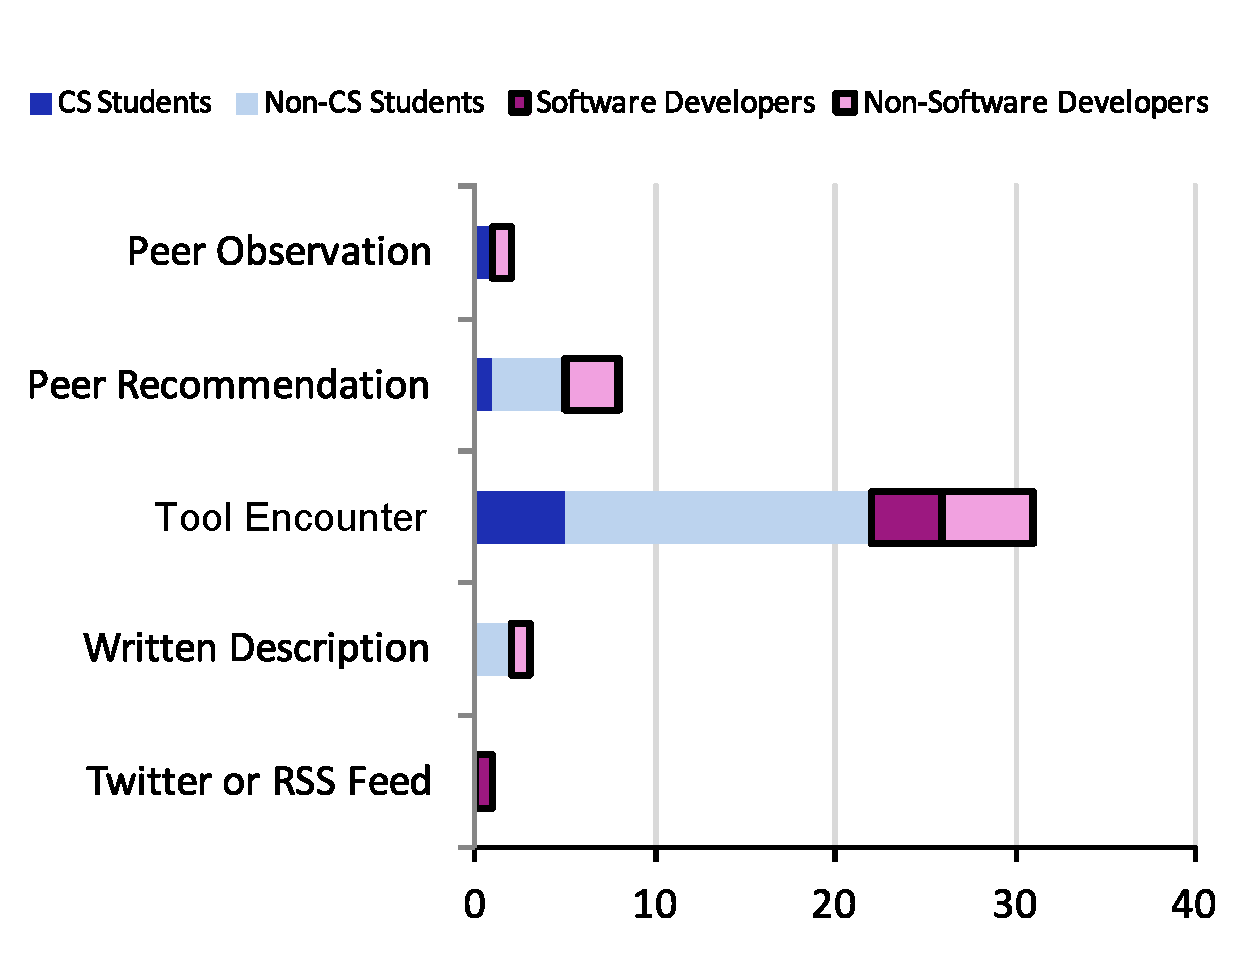
\includegraphics[width=\columnwidth]{freq.eps}
 	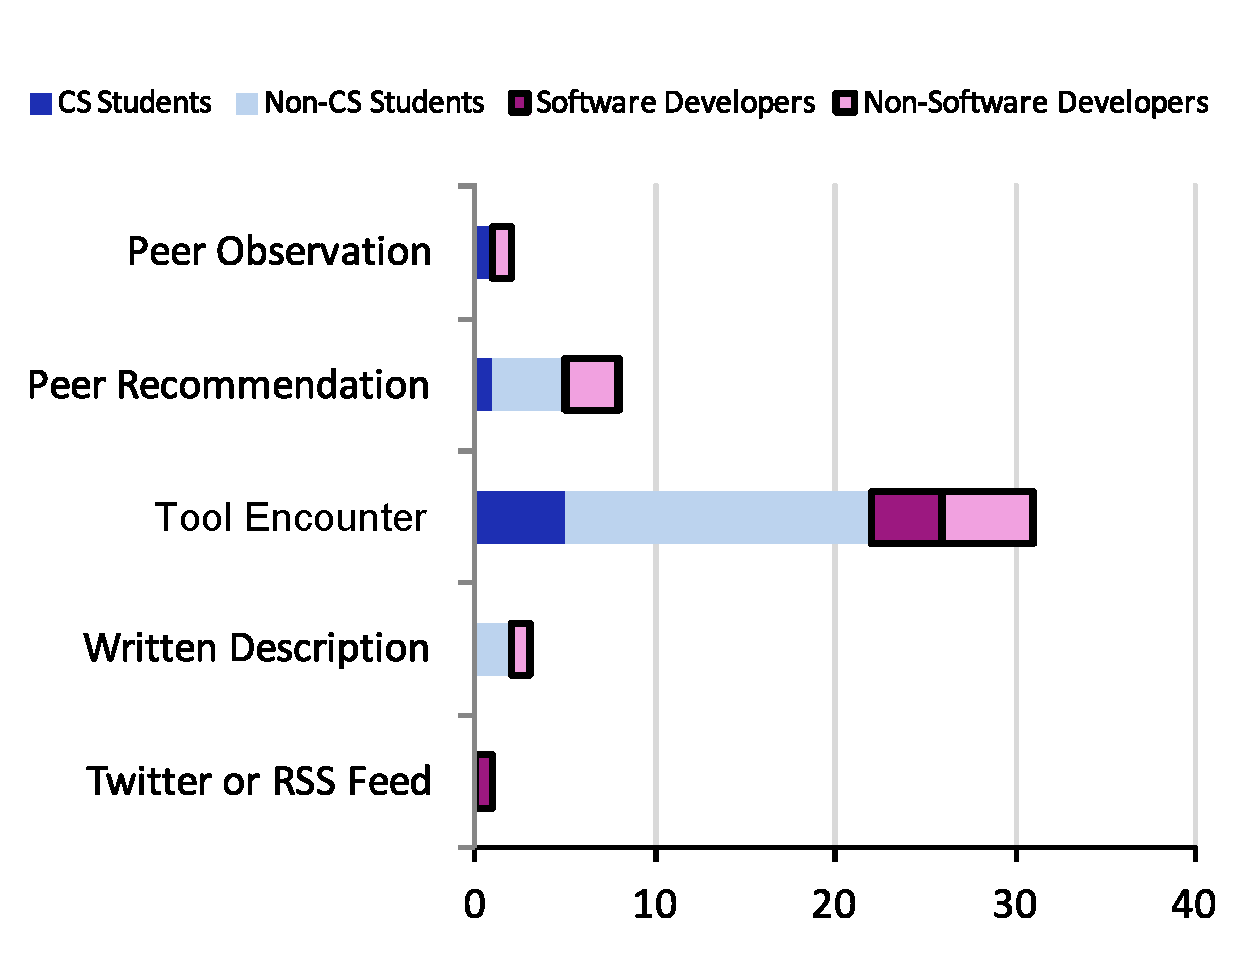
\includegraphics[width=90mm]{freq}
 	\end{center}
 	\vspace{-5 mm} 
 	\caption{Histogram of the most frequent discovery modes in the diary study (n=28 participants)
	%see people_submitting_chance_reports.
	}\label{fig:freq}
\end{figure}



\definecolor{sbBlue}{RGB}{29,47,179}
\definecolor{sbPurple}{RGB}{241,161,224}

\sethlcolor{sbBlue}

\noindent
To estimate how often peer interaction occurs, we measured how many
times participants' reported discovering a tool via peer interaction.
Figure~\ref{fig:freq} shows the frequency of each discovery mode.
For example, there were two reports of peer observation: one (in blue \hl{~}) 
\sethlcolor{sbPurple}
from a computer science co-op student and the other one (in pink \hl{~}) from a non-software developer.
Note that no ``Tutorial'' or ``Discussion Thread'' bars are shown 
because no participant submitted this type of discovery report. 

Figure~\ref{fig:freq} shows that participants reported tool encounter more frequently than any other mode of discovery, 
consistent with the findings in our interviews (Figure~\ref{tab:discoveryTypes}). 
The figure also shows that participants experience \discpush more frequently than \discpull,
in contrast to our interview findings (Figure~\ref{tab:discoveryTypes}). 
If we assume that all participants reported all instances of peer recommendation,
this data suggests that the average software user will discover a new tool via 
peer recommendation about once every 2 months. %(76*35 / 8) / 8 
If we make the same assumptions about peer observation,
the data suggests that the average software users will discover a new tool
via peer observation only about once every 8 months.
These projections are even less frequent than our interviewees' estimates of 
learning via peer interaction (Section~\ref{sec:frequency}).

 \begin{figure}[t]
 	\centering
 	\begin{center}
% 	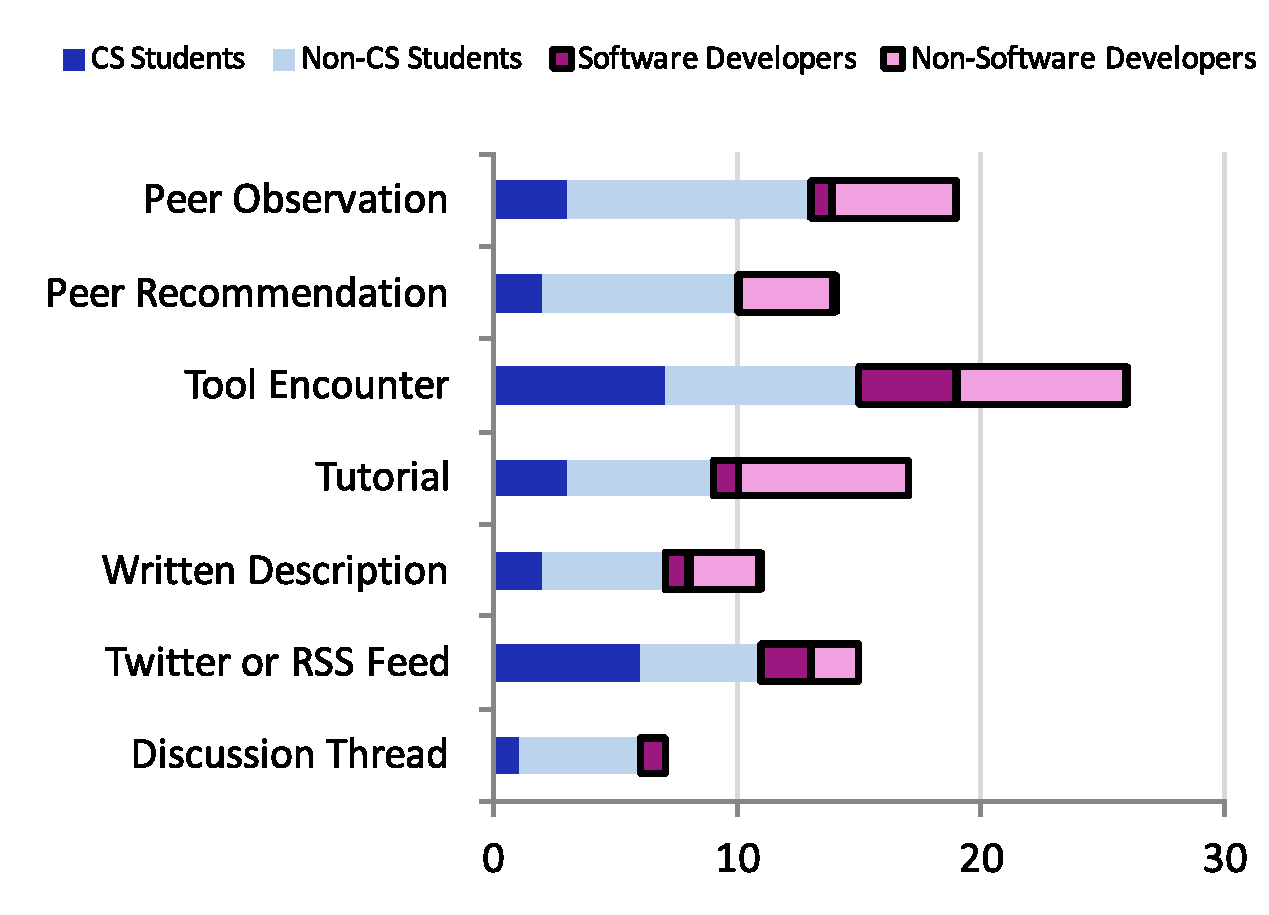
\includegraphics[width=\columnwidth]{effectiveness.eps}
 	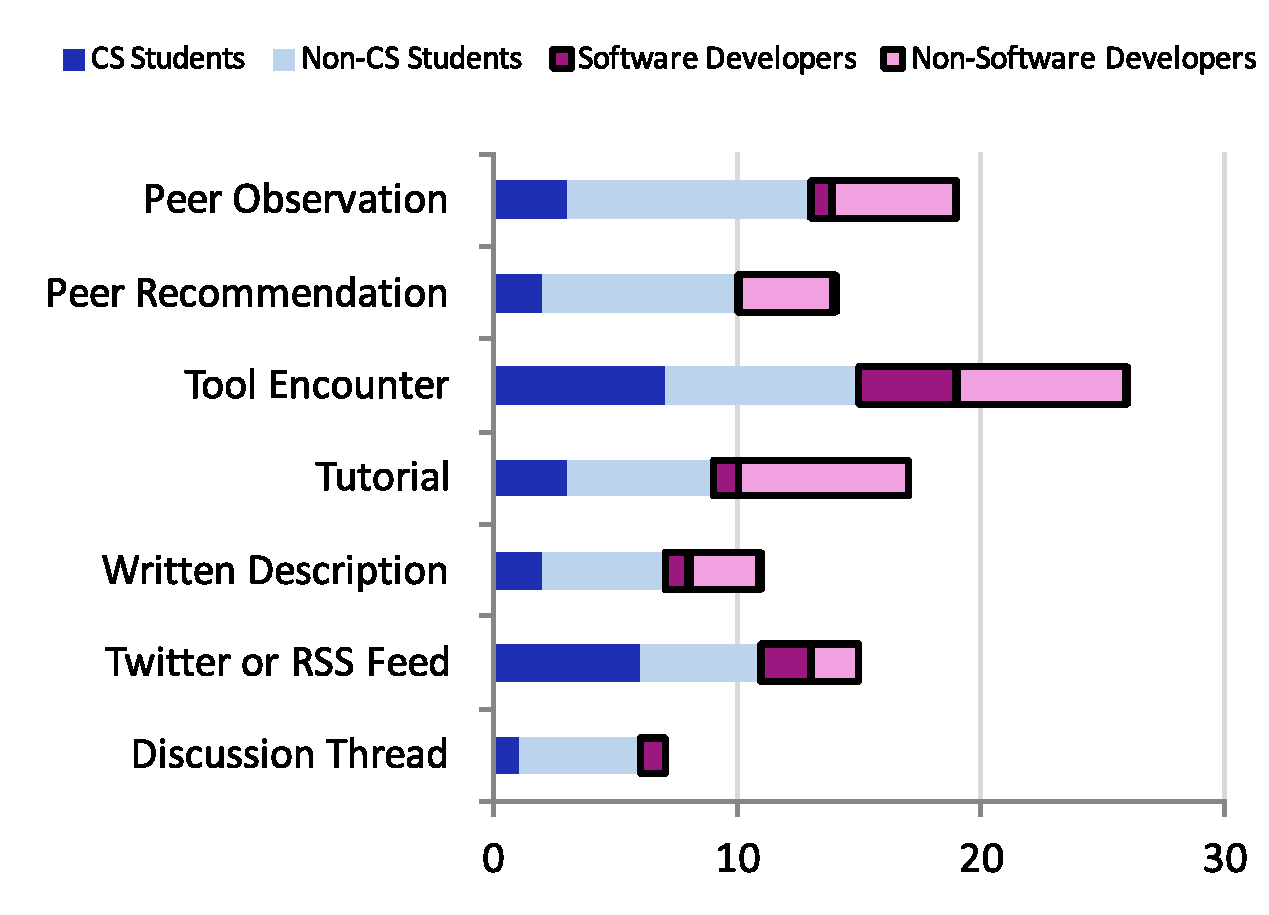
\includegraphics[width=90mm]{effectiveness}
 	\end{center}
 	\vspace{-5 mm}
 	\caption{Histogram of the most effective discovery mode reported in the diary study (n=50 participants).}\label{fig:effectivemode}
 \end{figure}
 
\paragraph{Effectiveness.}

As with our first study, we wanted to estimate how effective each mode
of discovery is for adopting new tools.
In this study, we did this in two ways.

First, we estimated effectiveness in the same way that 
we did in the interviews, by asking participants' to
rank the modes from most effective to least effective in their
post-study questionnaire.
Figure~\ref{fig:effectivemode} shows a histogram which
displays the top two highest ranked discovery modes for each participant.
When we asked this question in our interviews,
participants rated \discpull and \discpush as 
the most effective modes for discovering a new tool;
however, in this study, this was not the case.
%Because peer observation and peer recommendation were perceived as so effective
%among software developers, we hypothesized that it would also be perceived as
%effective among other kinds of computer users.
In particular, computer science students and software developers tended 
to rank tool encounter as their most effective mode. 
Interestingly, however, students who were not in computer science tended 
to rank \discpull and \discpush as their most effective modes. 

\begin{center}
\begin{table}[t]

\renewcommand{\arraystretch}{1.4} 

   \centering

	\topcaption{How often tools that were discovered using 
each discovery mode were used again six weeks later. n denotes the number of discoveries.}\label{tbl:reusing}
		
		
		\begin{tabularx}{100mm}{p{34mm}|r|r|r}
		\textbf{Discovery Modes}&\textbf{Frequently}&\textbf{Occasionally}&\textbf{Not at all}\\	
		\hline
    Peer Recommendation & 0\% (n=0)   & 80\% (n=4)  & 20\% (n=1)   \\\hline 
    Peer Observation    & 0\% (n=0)   & 100\% (n=1)   & 0\% (n=0)   \\\hline 
    Written Description & 0\% (n=0)   & 50\% (n=1)   & 50\% (n=1)   \\\hline 
    Tool Encounter      & 54\% (n=7)  & 31\% (n=4)   & 15\% (n=2)   \\ 		    
		\end{tabularx}
		
\end{table}
\end{center}

Second, we estimated effectiveness by asking participants whether
they were still using the discovered tools six weeks later.
More specifically, we asked each participant who submitted a tool discovery 
report six weeks later whether they were currently either 
(1) not using the tool at all, 
(2) using the tool rarely,
(3) using the tool weekly,
(4) using the tool once daily, or
(5) more than once daily.
%need to use word ``option'' somewhere here (done)
We collected a total of 21 reports (from 13 participants) 
where the participants chose one of the above options in using the tool.
%see still_using_modes in DB
For simplicity, we collapsed these five categories into three:
using the tool not at all (option 1),
using it occasionally (options 2 and 3), and
using it frequently (options 4 and 5).
Table~\ref{tbl:reusing} shows how often tools that were discovered using 
each discovery mode were used again six weeks later.
Note that ``Twitter/RSS Feed'' is not shown because there was only one 
discovery report submitted of this mode and no follow-up questionnaire was submitted.
%Interestingly, in our results, if we remove `not at all'' attribute, we observe that tutorial and peer recommendation discovers are the most frequently reused features.
As the table suggests, tools discovered by tool encounter may be used more 
frequently than tools discovered by other discovery modes. 
For example, seven out of thirteen tools discovered via tool encounter 
were used frequently six weeks later, 
whereas none of the five tools discovered by peer recommendation were used frequently. 

\paragraph{Discovery Frequency by Age and Experience.}

In our interview study, we noticed that more experienced programmers
tend to teach and learn via peer interaction less than junior programmers (Table~\ref{tbl:social}).
To investigate this further, we evaluated whether age, job length and experience is 
correlated with discovery frequency.
Using a Pearson correlation, we found that age is very weakly correlated with number of tool discoveries (r=-0.03 and n=47). 
Similarly, job length and experience show weak correlations with number of discoveries (r=-0.1 and n=55, and r=0.06 and n=55, respectively).
%TODO are these statistically significant? if so, p value? 
%Second, we compared discovery frequencies for discrete maturity groups, that is,
%students versus workers and student developers versus professional developers.
%Overall, there appears to be no 
%significant correlations between maturity and the number of tool discoveries.
%TODO use Wilcoxon signed-ranks here, unmatched (but need to find the data!)

\paragraph{Off-Task Time for Tool Discovery.}

In addition to understanding the effectiveness of discovery \contexts,
we are also interested in understanding the efficiency.
To do so, we analyzed how long participants spent 
learning about new tools, with respect to 
discovery modes and intent.
Table~\ref{tbl:context} shows our results, where
we notice two trends.
First, tool encounter tends to be the fastest discovery mode,
in terms of off-task time.
Second, finding a tool by chance was consistently the fastest
intent under which tools were discovered, across all modes.



\begin{table*}[t]

\renewcommand{\arraystretch}{1.4} 

   \centering

	\topcaption{The amount of off-task time (OTT) for different modes and intents for discovery. \textbf{n} represents the number of participants for the corresponding discovery mode and intent.}\label{tbl:context}
	
   \begin{tabularx}{\linewidth}{p{25mm}Xrr}
   		\textbf{Discovery Modes}&\textbf{Intent}&\textbf{n}&\textbf{OTT (sec)} \\
		
		\cline{1-4}
		%\hline
		
%Gail: should we include std dev?
%Emerson: probably not, since most n values are less than 5, so sddev doesn't make sense for those
		
    \multirow{3}[1]{*}{Peer Observation} & Discovered the tool by chance & 2     & 240   \\
          & Had problem, looked for a tool to solve & 0     & .    \\
          & In process of learning to use the software & 0     & .  \\
%          & other & 0     & .     & . \\
		
		\cline{1-4}
		%\hline
		
    \multirow{3}[0]{*}{Peer Rec.} & Discovered the tool by chance & 8     & 97    \\
          & Had problem, looked for a tool to solve & 22    & 410    \\
          & In process of learning to use the software & 7     & 930 \\
%          & other & 0     & .     & . \\
    
    \cline{1-4}
    %\hline
    		
    \multirow{3}[0]{*}{Tool Encounter} & Discovered the tool by chance & 31    & 26 \\
          & Had problem, looked for a tool to solve & 21    & 245    \\
          & In process of learning to use the software & 5     & 533   \\
%          & other & 1     & 0     & (1, 100\%) \\

   \cline{1-4}
   %\hline
    \multirow{3}[0]{*}{Written Desc.} & Discovered the tool by chance & 3     & 120   \\
          & Had problem, looked for a tool to solve & 40    & 753   \\
          & In process of learning to use the software & 4     & 680  \\
%          & other & 1     & 30    & (0, 0\%) \\

    \cline{1-4}
    %\hline
    \multirow{3}[0]{*}{Discussion Thread} & Discovered the tool by chance & 0     & .  \\
          & Had problem, looked for a tool to solve & 4     & 390   \\
          & In process of learning to use the software & 1     & 1200  \\
%          & other & 0     & .     & . \\

		\cline{1-4}
    %\hline
    \multirow{3}[0]{*}{Twitter/RSS Feed} & Discovered the tool by chance & 1     & 60   \\
          & Had problem, looked for a tool to solve & 0     & .   \\
          & In process of learning to use the software & 0     & .   \\
%          & other & 0     & .     & . \\				        
	\end{tabularx}
\end{table*}

\subsubsection{Threats to Validity}

\noindent
Although in this diary study we attempted to strengthen and generalize
the results of the interview study, there are still several
threats to the validity of the diary study that the reader
should consider when interpreting our results.
One threat was that, in follow-up emails, some participants noted that 
they made mistakes when categorizing a discovery by mode.
We attempted to mitigate this threat by having three raters 
re-code the data based on the remainder
of the discovery report (Section~\ref{sec:cleaning}).
Another threat is that the study may suffer from sampling bias because participants were 
not representative of all software users, in part because 
participants were all working in British Columbia, Canada.
A third threat is that, because participants 
sent tool discovery reports at their leisure, 
they may not have been motivated to write especially detailed reports,
reducing the fidelity of our results.
We tried to mitigate this thread by asking for additional information via
email, when necessary.
Another consequence of having participants report tool discoveries
is that it probably made participants especially reflective about the tools
they used, thereby increasing the probability that they would 
use the tool again at some point in the future.
Finally, participants' self-estimates of the elapsed time it 
took to discover a tool may not have reflected the wall-clock time
to discover the tool, a phenomenon that has been observed
in experimental psychology~\cite{huttenlocher1990reports}.
While the time estimate may not be accurate to the actual elapsed time,
if the inaccuracy is consistent across all \contexts,
we can still reasonably compare the time estimates against one another.

% Was there evidene for these?
% -Implicitly hotkeys are a barrier when doing this remotedly.
% -Generally, this says that live interaction is pretty rich!
% -The GUI is really a barrier; it works better on the command line (see
% Twidale05)

% \subsection{Other Interesting Bits}
% 
% ``In terms of tools that I already know and use, that learning comes largely
% through \discpull and \discpush\ldots especially tools for which I
% am no longer in the habit of actively expanding  my knowledge of.''
% That's interesting - people don't expand their knowledge of the tools they
% already know like IDEs and editors, because it's so hard to switch editors. 
% In the age of not wanting to switch editors, this seems to be a strong learning
% strategy.
% 
% Sometimes no advantage is given in the recommendation,
% so the author has to guess.
% This allows people to discover on their own.
% -Ivan: didn't specify whether synchronize was better
% -maybe Paul said this too?
% This conceivably has an impact on tool development.
% 	
% Two step process: discover, then follow up learn
% 
% There seemed to be a role of screencasts/videos for filling the void left by
% little human-human interaction.
% 
% Config file comparison/check out.
% 	-Gabe, who looks into others'
% 	-Hank, who keeps is home directory in a git repo
% 
% Rather than at-work recommendations, people occasionally found them socially
% (friends) or at meetings (user groups)

\subsection{Study Comparison}\label{sec:studyComparison}

In both our interview and our diary study, tool encounters dominated
as the most frequent way that software users discovered new tools,
both for programmers and other types of software users.
\Discovery was rarely reported in either study, both relative to 
tool encounters and in absolute terms; based on the diary study, \discovery
would only occur every few months.
\Discovery may be even rarer than we thought after conducting the interview study; 
even though 
we had about four times as many participants in
the diary study than in the interview study, we only collected about
a quarter as many episodes of \discovery in the diary study.

The assessed effectiveness of \discovery was not consistent between the studies.
In the interview study, it appeared clear that programmers believed that
\discovery was effective, but in the diary study, 
programmers (and other workers) did not rate it as especially effective. 
We believe this disagreement probably arises partly from differences
between the groups of participants, but also partly from differences between
how participants interpreted ``effectiveness'' in the two studies.
Further research is necessary in a more controlled setting to evaluate
the effectiveness of the various discovery modes.
%-use 6 weeks later, although numbers small, suggest that it was really effective

In our interview study, participants' remarks suggested that tool learning may decline with
age and experience, yet the diary study did not show any substantial 
correlations between such maturity measures and the number of tools discovered.
This agrees with previous work on technology learning in the workplace~\cite{brooke},
which suggests that there is a perception that older technology workers
are less able to cope with new technology, even when research suggests
the opposite~\cite{morrison}.
Indeed, our second study suggests that learning, at least in terms of software tools,
continues unabated throughout information workers' careers.

\section{Implications}\label{sec:discussion}

\noindent
While preliminary, our results have several implications.
We discuss four of them in this section: how software
environments can make it easier for users to discover tools from peers,
how teams can encourage \discovery,
implications for the design of recommender systems,
and methodological implications.

\subsection{Improving Tool Discoverability}\label{sec:discoverability}

\noindent
Our diary study suggests that users discover new tools 
at all levels of experience, underscoring the importance of
discoverability for all types of users.
We suggest that there are at least two ways toolsmiths can make
tools more discoverable, so that when users interact, \discovery is 
more likely to be successful.

\paraHead{Noticeable Causes.} If the manner in which a tool is used can be
easily observed, then an observing user is more likely to
both recognize that a tool was used and, implicitly, know how the tool is used.
A positive example of such a tool --- and one mentioned by several
programmers in our study --- is Eclipse's Open Type dialog box, which
shows a noticeable dialog box used for searching.
Hotkeys, used in many software environments so that
users can quickly invoke commands, such as \texttt{Ctrl+]} in Microsoft Word to increase text size, 
are a negative example because the
keys that are pressed are typically not visible on the screen.
One solution is to show the keys that are pressed on the screen for
a few seconds.

% \begin{figure}[t]
% 	\centering
% 	\begin{center}
% 	\includegraphics[width=\columnwidth]{emacs}
% 	\end{center}
% 	\caption{The emacs environment, showing the lower left that the keyboard
% 	sequence \texttt{Ctrl-c Ctrl-x} has been pressed.}\label{fig:emacs}
% \end{figure}

\paraHead{Noticeable Effects.} 
In addition to making the causes of a tool invocation obvious, \discovery may
be facilitated if the effects of a tool are clear.
This is a collaborative extension of Nielsen's ``visibility of system status'' 
usability heuristic~\cite{nielsenBook}.
Eclipse's Organize Imports command is an example of a tool that may not have
noticeable effects; the tool automatically adds and removes import statements
from Java files, but if those statements are not visible on screen, then an
observer may not notice the effect of running the command.
Another counter example is Microsoft Powerpoint's ``Set Layout'' command, which may
not produce any obvious visual changes, yet links a slide to a slide template, so that
future changes to the template are reflected in the slide.

% the following is very nice, but it's not really about discovery, it's about 
%	observing how a tool is used, not that it exists (or at least increasing
% 	likelyhood of adoption, which is not what this section is about)
% \paraHead{Non-modal.}
% A user interface is modal when there are distinct modes where different user
% actions produce different results.
% For example, suppose that you are programming in Eclipse with a peer, and you
% notice that the running program stops at a breakpoint
% 
% As a negative example, consider running a program in debug mode in Eclipse. 
% In the interval between when a programmer runs the ``Debug'' command and
% sometime later when the program hits a breakpoint, the program is in an
% \emph{invisible mode}.
% Because the mode is invisible, an observing programmer may not associate the
% cause (the debug command) with the effect (stepping through a program at a
% breakpoint), and thus may not learn how to use the tool without asking.
% 
% 
% have long been recognized as problem for
% single-user environments because the user may make inadvertent errors when she
% forgets what mode she is in~\cite{raskin}.
% 
% Our research suggests that modal user interfaces can be harmful for
% multi-user environments, such as development environments during
% pair-programming, because they may interfere with \discovery.
% As a positive example, Eclipse's Open Type Dialog, has a prominent, simple user
% interface that is easily perceptible to observers.

\subsection{\DisCovery without Collocation}

\noindent
Our results from both studies suggest that \discovery is already
very rare.
As teams increasingly do more and more work in a remote fashion,
our section on barriers to \discovery imply that
it will become even more challenging for remote teammates to learn
tools from one another.

\paraHead{Remote Pair Programming.}
Several interviewees reported learning new tools via \discovery with
a peer by working at separate, remote workstations using
a screen-sharing program.
However, additional constraints have to be satisfied in order for such
\discovery to take place.
First, the pair needs some channel by which to ask ``what just happened?'', 
such as using instant messaging or an audio link.
Second, visible causes and effects are especially important during remote pair
programming, because implicit cues about how a tool is used, such as where a
programmer's fingers are on the keyboard or where a programmer is looking, are
absent. 
Third, programmers need a convenient, concise way to communicate about their
tools.
This third constraint is sometimes difficult to achieve.
For example, if the programmers choose to collaborate using Eclipse
and a tool requires several complicated steps to use, the teacher may be
forced to say ``first you click here, then here, then here, then type in
this,'' and so on. 
More elegantly, if the programmers choose to collaborate using an
environment with purely textual commands, like vim, the steps can be easily
represented as a series of brief commands.
Although we know of no equivalent of pair programming for general 
information workers, we believe that these constraints apply equally
to situations where remote information workers wish to learn from
their peers.

\paraHead{Learning from the Strengths of \DisCovery.}
In the future, we might expect that collocated \discovery will
decrease as teams become more distributed, while at the same time, 
micro-blogging (Twitter) and internet tutorials (screencasts) 
may be increasingly common.
However, both of these typically lack the qualities that make
\discovery effective, such as that \discovery takes place in the context 
in which the tools are used.
We view this as an opportunity: what can we learn from \discovery to make
other discovery \contexts more effective?

Twitter bears some similarity to \discpush in that
both are types of social discovery, yet few interviewees and 
zero participants in the diary study learned about tools via Twitter.
One reason that interviewees cited for Twitter being ineffective is lack of trust
in the sources and lack of relevance.
From the interviews, it appears what programmers meant by trust was that the
recommender (human or otherwise) requires some prior interaction with the
recommendation recipient, so that the programmer can estimate the recommender's knowledge and
skills.
Our studies suggest that trust and relevance might improve if the Twitter
messages originated from a trusted peer, someone that a software user works with
or has worked with in the past.
Rather than burdening the trusted peer with having to report whenever she
discovers a new tool, we imagine a system that automatically notices when she
uses a novel tool and generates microblog messages to coworkers on her behalf.

Several interviewees reported watching screencasts that were professionally
produced (e.g., \url{peepcode.com}).
Although watching screencasts is similar to \discpull, participants reported
that the tools used in screencasts may not be very relevant, presumably because
the people who made the professional screencasts did not have working
styles that aligned with individual interviewees' working styles.
Because peers are more likely to have similar working styles, a
screencast produced by a peer is potentially more relevant.
However, no participant in either study reported watching a screencast produced by a peer.
We suspect that the reason that software users do not make screencasts for their
peers is that the costs (the time required for recording, editing, and distributing) are
too high compared to the benefits (the possibility of a peer discovering a
tool).
\lsub, from the first study, hinted at this; ``I wish people did make more screencasts; they're a
pain in the ass to make.''
Better tool support for creation, editing, and distribution of screencasts may
make it more likely that software users will produce screencasts for their peers,
improving screencasts' effectiveness.

\subsection{Design of Recommender Systems}

\noindent
Systems that can recommend relevant tools are one approach to helping users
learn new tools.
Past systems have included the controversial Clippy 
(\url{http://www.microsoft.com/presspass/features/2001/apr01/04-11clippy.mspx}),
which takes the form of a virtual talking paperclip to recommend features of
Microsoft Word.
In what follows, we discuss two design considerations for such systems.

\paraHead{Trust.} Interviewees' frequent refrain of the necessity of trust
underscores its importance in a recommender system for tools. 
\ksub, when asked about his opinion of a potential recommender system, summed up
the problem as:


\begin{quote}
Honestly; I bet the [recommender system] would have better success rate [than
a peer] at recommending things that I would like, but that doesn't mean that I
would trust the [recommender system] more.
\end{quote}

Since trust appears to be a by-product of prior social interactions during \discovery,
how can a recommender system without any prior interactions be trusted
at all?

One way is to borrow trust from a trusted peer. 
Specifically, rather than saying, ``You should use this tool,'' a
system could instead say, ``your friend, John, also uses the
tool, so you should check it out,''\footnote{A direct quote from \jsub.} making
a recommendation based on what your peers are using.
In this way, the user no longer needs to have trust in the recommendation
system beyond that it is accurately recording her teams' tool usage, and
instead the user can rely on trust between teammates~\cite{murphyHill12b}.
This was the approach taken by Toolbox, where the system
looked for expert tool users, requested that these experts write down
descriptions of the tools, and published the descriptions as newsletters in
the expert's organization~\cite{maltzahn}.
We have sketched such a system using screencasts 
for software developers in a recent paper~\cite{murphyHill12b}.

Another way to avoid the trust dilemma is to sidestep it altogether.
\csub mentioned that a recommender system might be acceptable if it makes ``you
feel like you discovered it.''
Implementing such a recommender system would require a more subtle interface
than the traditional ``you should use this tool'' interface.

\paraHead{Beyond \DisCovery.}
Although recommender systems may have been originally inspired by
recommendations offered by trusted peers, the design of recommender systems
could benefit by going beyond traditional \discpush by closely
examining the limitations of \discovery.

Interviewees noted that \discovery does not work when the peers are under time
pressure because the teacher feels like he cannot respond to the learner's
question, ``what did you just do?''
If a recommender system can capture experts' usage of tools, that
usage can be played back repeatedly and at the convenience of a user who
wants to learn a tool.

\Discovery has other limits: just because a single software user uses a tool,
that does not mean that other users would find it useful.
However, if many users find a tool useful, it is more likely that a
user who does not yet know it will also find it useful.
Recommender systems could gather, summarize, and present the usage habits of
the community, rather than relying on only one individual.
This is the approach taken by some recommender systems, such as
CommunityCommands~\cite{matejka09}.

Interviewees noted that sometimes they did not make recommendations because they
did not think that their peer was ready to appreciate the usefulness of a tool.
One way that recommender systems could deal with this would be to explicitly
model how specific users learn by monitoring what tools they know,
and inferring discovery patterns and contexts. 
A recommender system could then recommend appropriate tools at the right time
and in the right context, and therefore not only make relevant
recommendations, but also improve the likelihood that the user will
adopt the tool.

\subsection{Methodological Implications}

\paraHead{Individual Interpretation Differences.}
As we speculated about in Section~\ref{sec:studyComparison},
different participants may have had different interpretations of the word
``effectiveness.''
They may have also had different interpretations of 
the meaning of different \contexts of discovery (Table~\ref{tbl:methods}).
Because we re-categorized discovery reports based on our own intended meaning, 
the impact of this potential issue was limited.
Nonetheless, in future studies we intend to provide richer
definitions to participants, congruent with the complexity we observed of each
\context in this study.

\paraHead{Generalizability.}
As we mentioned in the threats sections for both studies,
the studies have limited generalizability due in part to 
the number of instances of \discovery captured.
In retrospect, the low number of instances that we were able to capture were 
inevitable, given that \discovery apparently occurs so infrequently.
A much longer-term journal study might have been able to capture more instances,
but at the same time participants may have been unwilling to keep a diary
of their tool discoveries for much longer than a week.
One alternative would have been to have them focus on \discovery only,
rather than reporting all \contexts of tool discoveries.
A focus on \discovery may, however, encourage more social tool discoveries than
would normally take place.
Ultimately, our goal of capturing realistic \discovery in the field remains a 
challenge that is difficult to overcome with any methodology.

\paraHead{Within-Group Comparisons.}
As a consequence of the somewhat low number of instances of \discovery,
our ability to make reliable within-group comparisons was limited.
For example, in Table~\ref{tbl:reusing}, we compared how different 
discovery \contexts correlated with participants' likelihood to continue to use a tool
six-weeks after the initial discovery.
In that table, most cells have four or fewer instances of tool discovery,
making it difficult to draw strong conclusions about the effectiveness of 
different \contexts.

One methodology that would enable more reliable comparisons between
groups would be a laboratory experiment.
For instance, we could teach several undergraduate
students about a given new tool, exposing groups to different 
discovery \contexts, then ask them
several weeks later if they were still using the tool.
Fortunately, based on the results from the present studies, 
we can craft several realistic learning scenarios for such an experiment.

% 
% Screencasts.
% Twitter.
% Blogs.
% Commit notifications.
% But what they're lacking: trust, context, ease-of-communication.
% 
% 
% How, then, can we facilitate it, so that \discovery occurs more frequently? 

% The characteristics of the kind of learning described by Cockburn and Williams
% have implications beyond pair programming.
% For instance, as software is developed on a global scale, teams become more and
% more distributed, reducing the discovery of tools during traditional pair
% programming.
% Thus, understanding how this type of learning takes place may help us
% facilitate tool discovery, by supporting its characteristics, in distributed
% development. 

% So, how could a distributed team share tool knowledge effectively?
% One answer is the notification produced by Toolbox, which ``periodically
% advertises the ToolBox services to the community by sending out weekly email
% newsletters''~\cite{maltzahn}.
% Our subjects' distrust for advertising in the study described here, coupled
% with our previous experience where programmers had difficulty in understanding
% textual recommendations~\cite{apple}, suggests that this approach will not be
% as effective as traditional peer discovery.
% %non-contextual, also
% An alternative approach for presenting tool knowledge was suggested by \lsub:
% 
% \begin{quote}
% I wish people did make more screencasts; they're a pain in the ass to
% make\ldots
% If there were ways that people could, if they were working with some tool on
% some particular task, if there were a way to very easily capture what they were
% doing, something akin to the way you record macros in [Microsoft] Excel\ldots
% where you say, `computer, watch what I'm doing,' and it's all done and you have 
% something you can package up and send as one.  
% If they make it that easy, where the person making
% the material doesn't have to set out to make that material, but instead they're
% using a feature where\ldots [the tool says] `if you like this tool, would you
% mind us recording you using it?
% We'll anonymize the text you're working on.' \ldots 
% There's a lot of people who
% get excited about what they do and they would love showing somebody\ldots   
% If it could be as easy as, `Hey, what are you doing? Press a green
% button to go and a red button to stop' and it gets posted and indexed and
% tagged\ldots that would be great.
% \end{quote}
% 
% \noindent
% Indeed, our study suggests that this is a good substitute for traditional
% \discpush: it builds on the social aspect of discovery; it strives to
% avoid being distracting; it maintains some of the contextual benefits of
% \discovery, and it leverages screencasts, which several subjects 
% reported using to discover new tools (\csub, \gsub, \lsub).
% Extending \lsub's example slightly, the social impact may be enhanced by
% leveraging existing social networks, for example, by posting the screencast as
% a blog post, a Facebook post, a tweet, or an email.  

\section{Conclusion}

\noindent
A wide variety of tools have been built to help software users, but individuals
must necessarily discover those tools before they can be used.
While there are many ways that users discover useful tools, 
the interview study described in this paper suggested that
\discovery is effective but rare. 
Our diary study suggested that tool encounters occur
more frequently than \discovery.
Successful \discovery occurs in social contexts where users have 
peers that they can observe, such as in a collocated team, 
but also in technical contexts where such observations are 
facilitated, such as when one user can see the outcome of another
user's tool use.
Towards our goal of encouraging software users to 
discover useful tools more successfully and more frequently,
our results open new possibilities to make existing tools and environments more
discoverable and distributed collaboration more effective.


\idrg{page numbers}

\section*{Acknowledgments}

\noindent
Thanks to the interview participants.
Thanks also to
Christian Bird,
Andrew Black,
Kellogg Booth,
Giuseppe Carenini,
Cristina Conati,
Nando de Freitas,
William Griswold,
Ciar\'an Llachlan Leavitt,
Karon MacLean,
Nancy Perry,
Kenneth Reeder,
Martin Robillard,
Claudia Rocha,
Martin Schulz,
Jonathan Sillito,
Laurie Williams,
Phil Winne,
Petcharat Viriyakattiyaporn,
and the members of the Software Practices Lab and
Interaction Design Reading Group at UBC
for their help, during various stages of this research.
This work was supported by the IBM, NSERC,
as well as 
by the National Science Foundation under grant number 1252995.

\bibliographystyle{abbrv}
\bibliography{references}

\section*{Appendix}\label{sec:app1}

\noindent
On the following pages, you will find:

\begin{itemize}
  \item
  	the interview script used in the first 
  	study (Section~\ref{sec:thefirststudy});
  \item
  	the discovery report (recall that we asked participants to report ``features,'' although
  	we use the word ``tools'' through this paper) used by participants in the 
  	diary study (Section~\ref{sec:thesecondstudy}); and
  \item
  	the final questionnaire used by participants in the
  	diary study (Section~\ref{sec:thesecondstudy}).
\end{itemize}

\noindent	
Text in gray was de-emphasized to improve readability 
for the interviewer.

%Gail: this script should be reproduced more cleanly
%Emerson: actually it's the original embedded. some text is gray, as it was in the original,
%			because it made the document easier for me to read. I can't easily change this text
%			to black, since I'm not sure where the original word doc is.
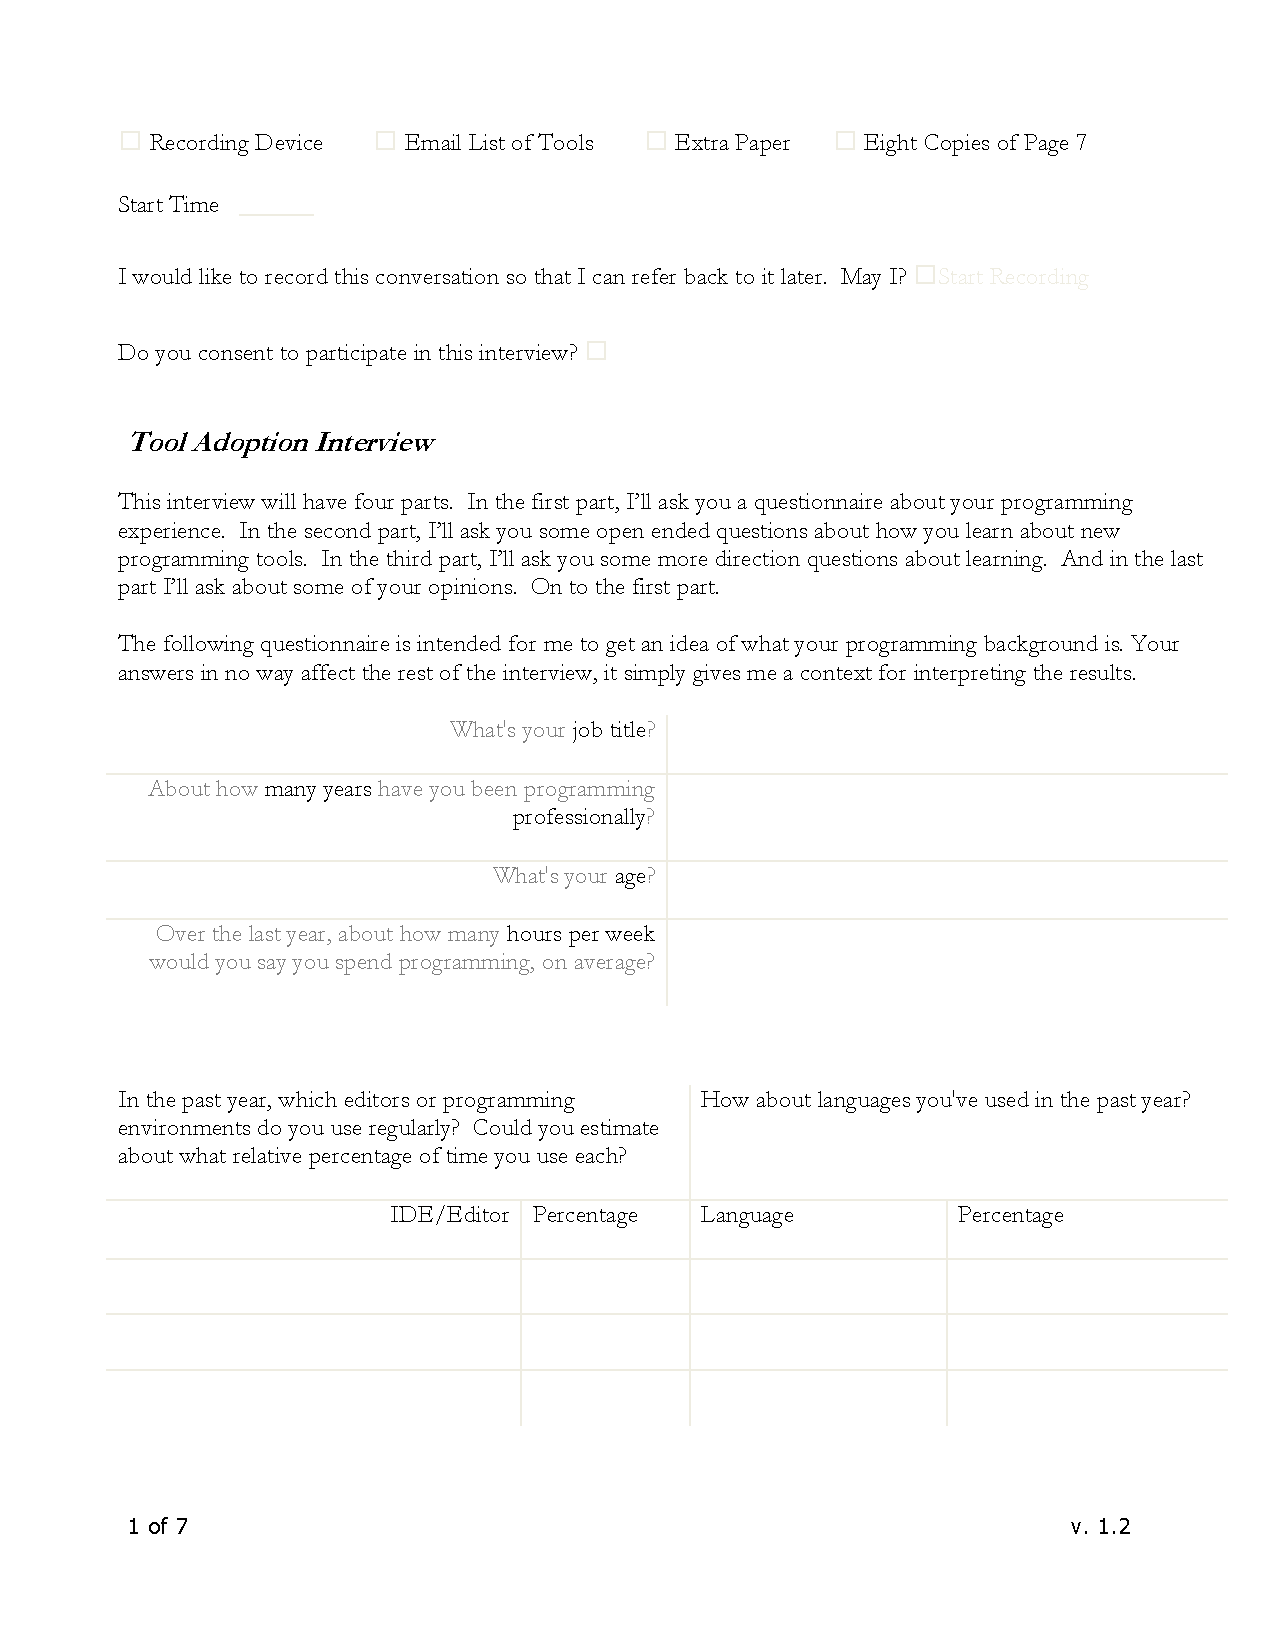
\includepdf[pages=-,frame=true,noautoscale=true,scale=0.6]{adoption_interview_script.pdf}
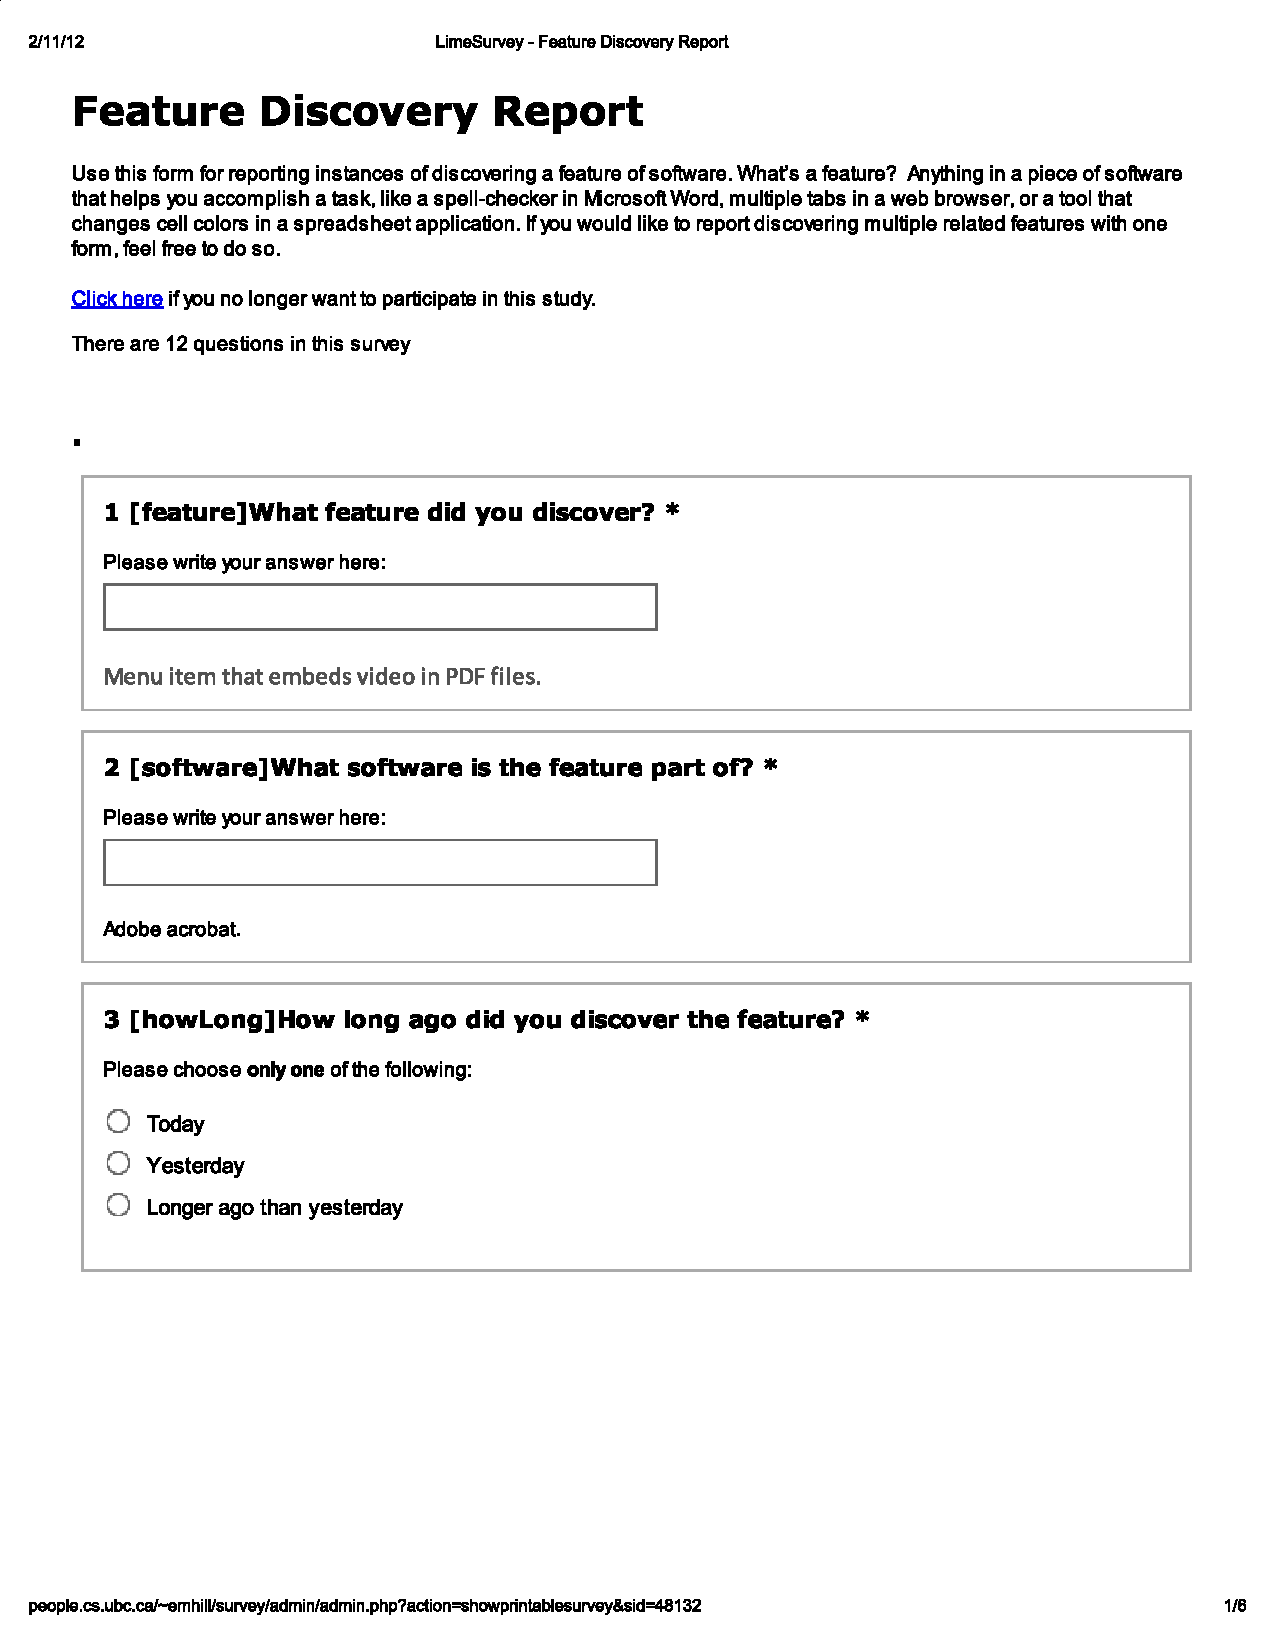
\includepdf[pages=1-5,frame=true,noautoscale=true,scale=0.6]{FeatureDiscoveryReport.pdf}
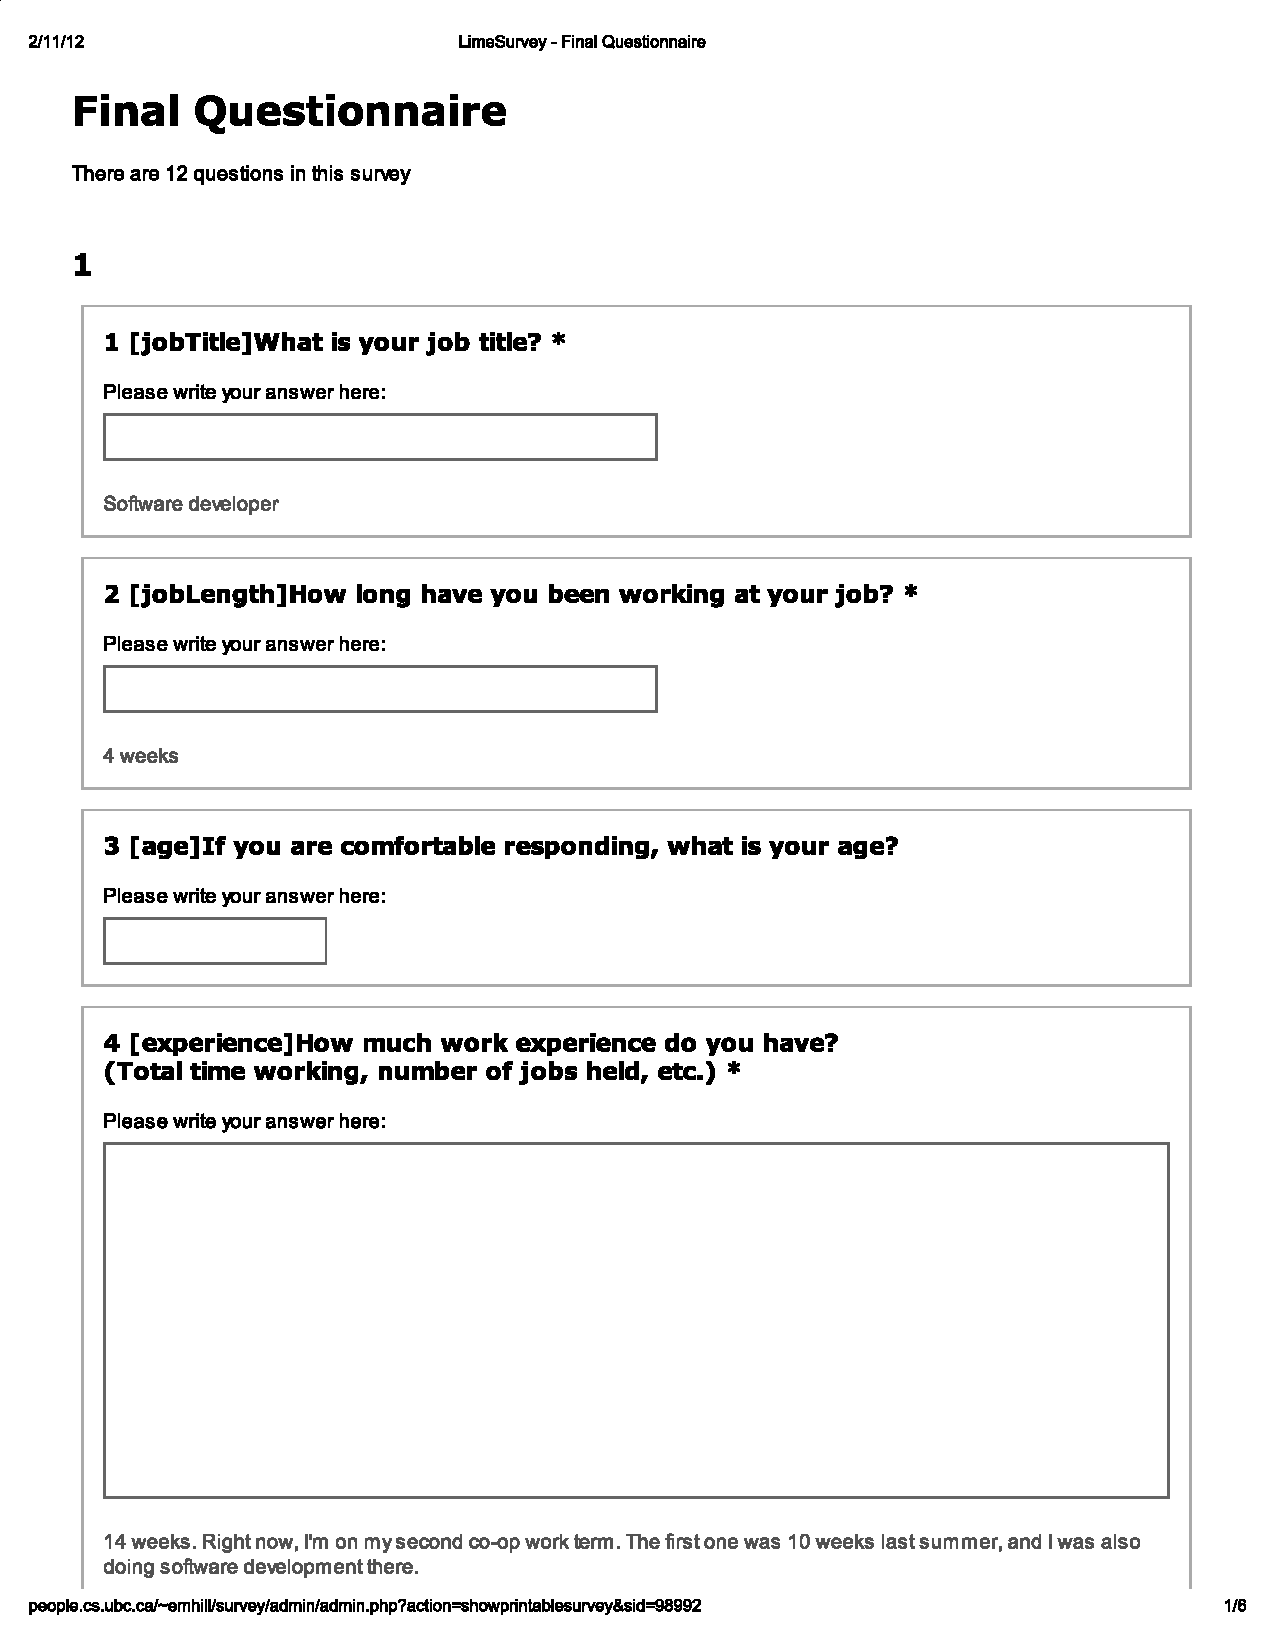
\includepdf[pages=1-5,frame=true,noautoscale=true,scale=0.6]{FinalQuestionnaire.pdf}

\end{document}